\chapter{WorkshopAR - Implementation Process \label{ch5}}

The previous chapter detailed the architectural design of \emph{WorkshopAR}, that is, the main ideas and decisions taken to fulfil the goals proposed for the software development, and the
efforts done to align the technical aspects of the project with the educational goals present in the research. The chapter also identified key components of the development process to
follow and proposed an overall plan for the implementation of the software.

This chapter will continue the technical analysis of the project by exploring the implementation process. This analysis will highlight the research done to identify and propose a suitable
interaction design for the context around \emph{WorkshopAR}, the evolving tendencies in the implementation of \ac{AR} experiences and all the information regarding good and bad practices
that had been found in the literature.

It will also offer a comparison between the plans and ideas proposed in the architectural design against the actual implementation of the software, identifying the reasoning behind such
changes and how the context and circumstances of the development shaped the final product.

Finally, this chapter will detail the software development process used. The process went through two development iterations complemented by testing procedures and early validations. There
was also an important effort to integrate the development of the tool with the case study, and the software constantly evolved with the particularities of the course and the educational
needs of the students.

Chapter \ref{ch3} detailed the reasoning behind the chosen development methodology, explaining how an iterative approach allowed for experimentation and flexibility, and that it better
accommodated the constraints in time and resources found in the research, facilitating a \emph{just-enough} approach to architecture, design and implementation. As a result, \emph{WorkshopAR}
undertook a development process in two iteration cycles which  ended up with the testing and deployment of a prototype used for observation and data gathering. Both cycles were structured
around a design phase, an implementation phase and quick adjustments. In between iterations it was possible to allocate some time for data analysis and planification for the next cycle.

Iteration 1 focused on building and testing the functional \ac{AR} technology behind \emph{WorkshopAR}: the shared \ac{AR} space and the fundamental \ac{AR} interactions. The overall goal
was to explore the main use cycle of creating a \emph{digital room}, starting a session with other users and sharing visualisations of different digital objects. The in between testing and
analysis was used to better align WorkshopAR to the particularities of the Industry Project course, as well as incorporating key observations provided by initial test users.

Iteration 2 focused on providing the needed functionalities to fulfil the use cases identified in the architectural design process, those that provided most value to the users and the
research. A final analysis of the results was done to identify possible solutions to the issues and ideas generated from the data gathering, both at an implementation and design level.
There is also a discussion of possible future steps for \emph{WorkshopAR}, of how the software can evolve and the lessons learned for future or related scenarios.

The following sections will describe this implementation process and provide a post-mortem of the activity to promote discussion and analysis of the results. Section \ref{sec:5-1} will
first detail the research done as part of the interaction design of \emph{WorkshopAR}, research that informed the approach that the software was going to take in relation to \ac{AR}
technologies and how to implement a set of interactions for the collaborative and multi-platform tasks present in the context of the development. Section \ref{sec:5-2} will describe and
show the results of the development process, organising the analysis around the two iteration cycles described previously. Section 5\ref{sec:5-3} will act as a final analysis and
conclusion of the results of the implementation process, the development of WorkshopAR and for the technical section of the research in general.

\section{Interaction Design \label{sec:5-1}}

An important effort in the construction of \emph{WorkshopAR} was dedicated to the design of the interactive elements at the core of the experience. The interactions that received the most
attention during the design process can be classified in three:

\begin{itemize}
    \item Interactions with digital objects (user anchors, play models, annotations) in the \ac{AR} spaced created for the room.
    \item Social interactions between participants in relation to group management and the activities of the course.
    \item The controls of the tool itself, the individual components and the flow of the work session.
\end{itemize}

These interactions were prioritised because they represent the tools that \emph{WorkshopAR} uses to promote the behaviours and ideas around collaboration at the core of the objectives of
the project. It is important for the interaction design proposed to be as invisible as possible, without interfering too much in a negative way or hindering the academic work of the
students using the tool. In a similar light, the project also offers the opportunity to explore solutions to a variety of interaction problems associated with the use of AR in mobile
devices such as:

\begin{itemize}
    \item Simultaneous interaction with digital objects that are shared with other users.
    \item Organise and select information.
    \item Use and understand social cues from other users.
    \item Plan and organise tasks for a common objective.
    \item Jump from using the \ac{AR} application to any other external activity and vice versa.
\end{itemize}

The following section will explore all these aspects of the interaction design in two parts. The first part will focus on general \ac{AR} design and will detail the research done to
understand how to use mobile \ac{AR} devices in social and collaborative activities, and the user-guided design followed to identify the best approach to the overall \ac{AR} interactions
needed for the implementation of \emph{WorkshopAR}.

The second part of the section will detail the decisions taken for the top-down interactions implemented for \emph{WorkshopAR}, that is, the final implementation and user experience for
activities related to create a \emph{work session}, interact with the digital objects in the \emph{digital room} and structure the collaborative activities of the group using \emph{WorkshopAR}.

\subsection{Collaborative interactions in AR \label{sec:5-1-1}}

Successful implementations of \ac{AR} in everyday usage and production, such as those reported by \textcite{kowalewski_2017}, demonstrate the practical application of \ac{AR} in software
development. Furthermore, the availability of ready-to-use software like Manifest \parencite{nmanifest_2022} and the accessibility offered by end-user products like the Meta Quest 3
\parencite{meta_horizon_2025} highlight the need to consider any development within the broad spectrum of mixed realities as a product intended for the general consumer. This is why the
development of \emph{WorkshopAR}, although envisioned as a research prototype, aims for an implementation guided by a user-centred, human-centred design approach.

For a human-centred approach it is important to consider the requirements that are directly related to interactions of the end user with the core utility of the product and the context in
which they happen \parencite{boy_2017}. This general design goal is highly relevant for \emph{WorkshopAR} if seen as a product introducing \ac{AR} technology to the collaborative education
context. \ac{AR} technology remains relatively new to most consumers and most of them have little or no contact with it in their daily routines \parencite{chang_2023}. Consequently, users
have not yet developed a consistent digital literacy around these and similar technologies. Is equally uncommon, even for experienced users, to have any form of expectations about the
behaviour and allowed interactions of any development. Even when an application is deployed in a more recognisable platform, like a smartphone, the affordances and interaction methods that
the users are accustomed to may not be the same or may be entirely absent.

Several efforts have been made to create a shared language for developers to use in the interaction design of their applications, and to solve common problems with consistent approaches.
Research studies such as those conducted by \textcite{piumsomboon_2013,wobbrock_2009} have formulated and compiled an array of intuitive gestures tailored to various forms of \ac{AR} and
\ac{MR} interactions. These proposed sets of gestures encompass a broad spectrum of general interactions, ranging from object selection and manipulation to complex tasks like file browsing
and content editing. However, these studies worked  under the assumption of single-user interactions.

While some interactions may be the same in both scenarios, others are unique to multi-user settings. Moreover, it is important to note that collaboration is not a given characteristic of
multi-user scenarios. The objective of the research described in this section is to explore the particularities of collaborative interaction in \ac{AR}. Using the same user-centred
methodology proposed in the studies cited previously, the aim is to identify common tasks executed in a collaborative setting using different forms of \ac{AR} technology. Based on that,
the result is a proposed set of gestures that capture the most natural interactions that users perform and tend to converge to. The results were directly used as a design guideline for the
interaction design of \emph{WorkshopAR}, highlighting effective strategies to tackle tasks related to the use of AR in the collaborative scenario and the use of mobile devices as the focus
for deployment.

\subsubsection{Research Methodology \label{sec:5-1-1-1}}

The interaction design process was guided by a three-step procedure:

\begin{enumerate}
    \item Identification and selection of tasks.
    \item Data collection from participants proposing interactions for the identified tasks.
    \item Analysis of the collected data to identify convergent approaches, recurrent issues, and common behaviours.
\end{enumerate}

In total, 24 different participants were interviewed with a median age of 41 and standard deviation of 11. Of the participants, 66\% were women while 34\% were men. In terms of
demographics, 20\% of the participants were university students with careers mostly in design and computer science. The remaining participants were professionals in different fields like
IT, medicine, and administration.

Two different scenarios were designed for the test. In Scenario 1, participants were equipped with a smartphone in one hand, leaving the other hand one free to interact during each task.
Scenario 2 involved the use of a Microsoft HoloLens headset, which afforded the participants the freedom to use both hands. Figure \ref{fig:5-1} shows examples of each scenario.

\begin{figure}
    \centering{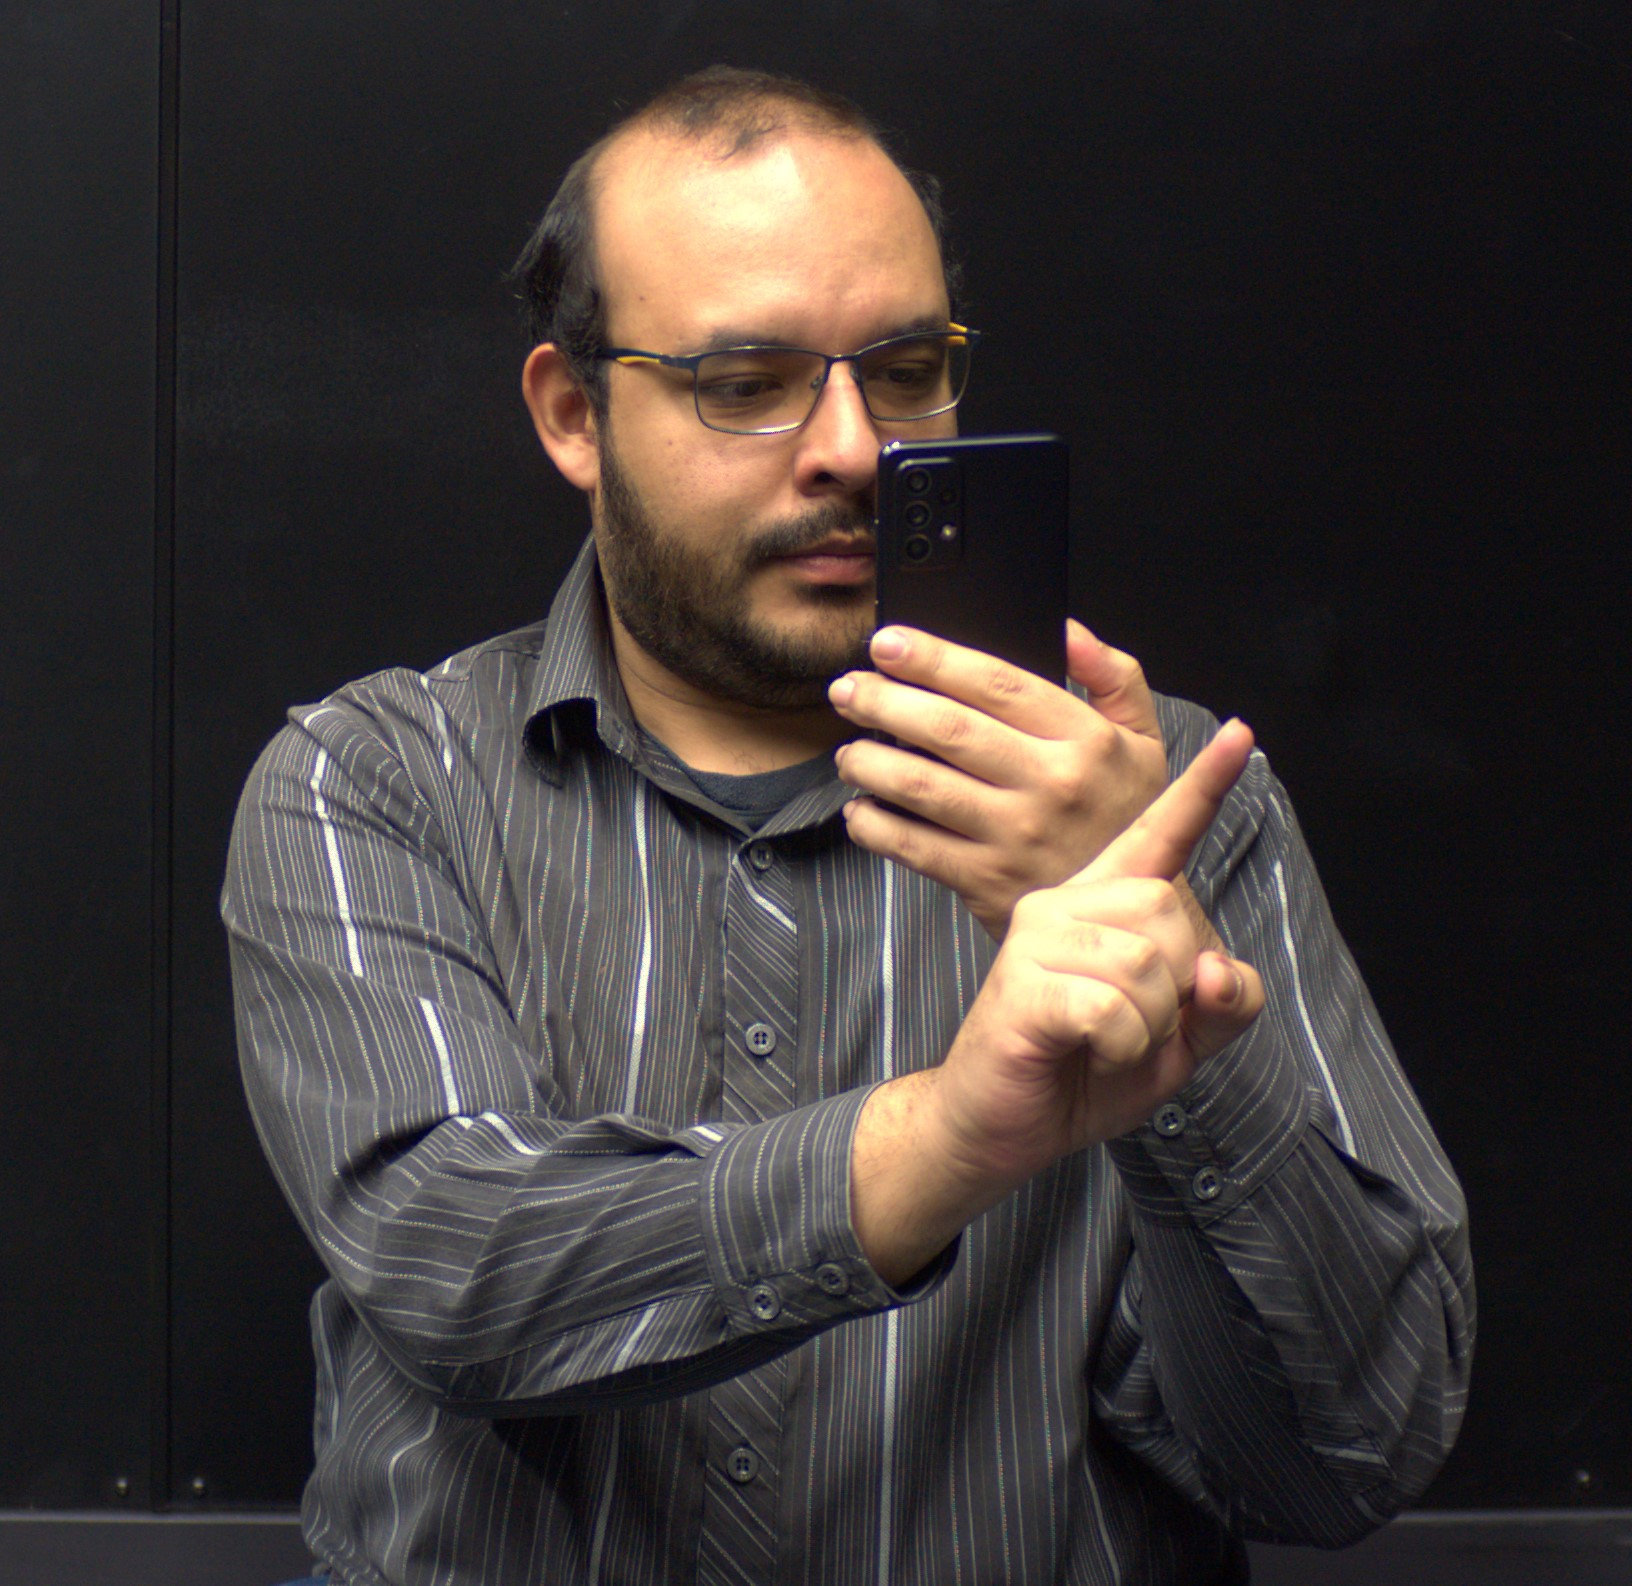
\includegraphics[alt={Figure 5.1a},width=0.49\textwidth,height=0.33\textheight]{figures/F5-1A.jpg}}
    \centering{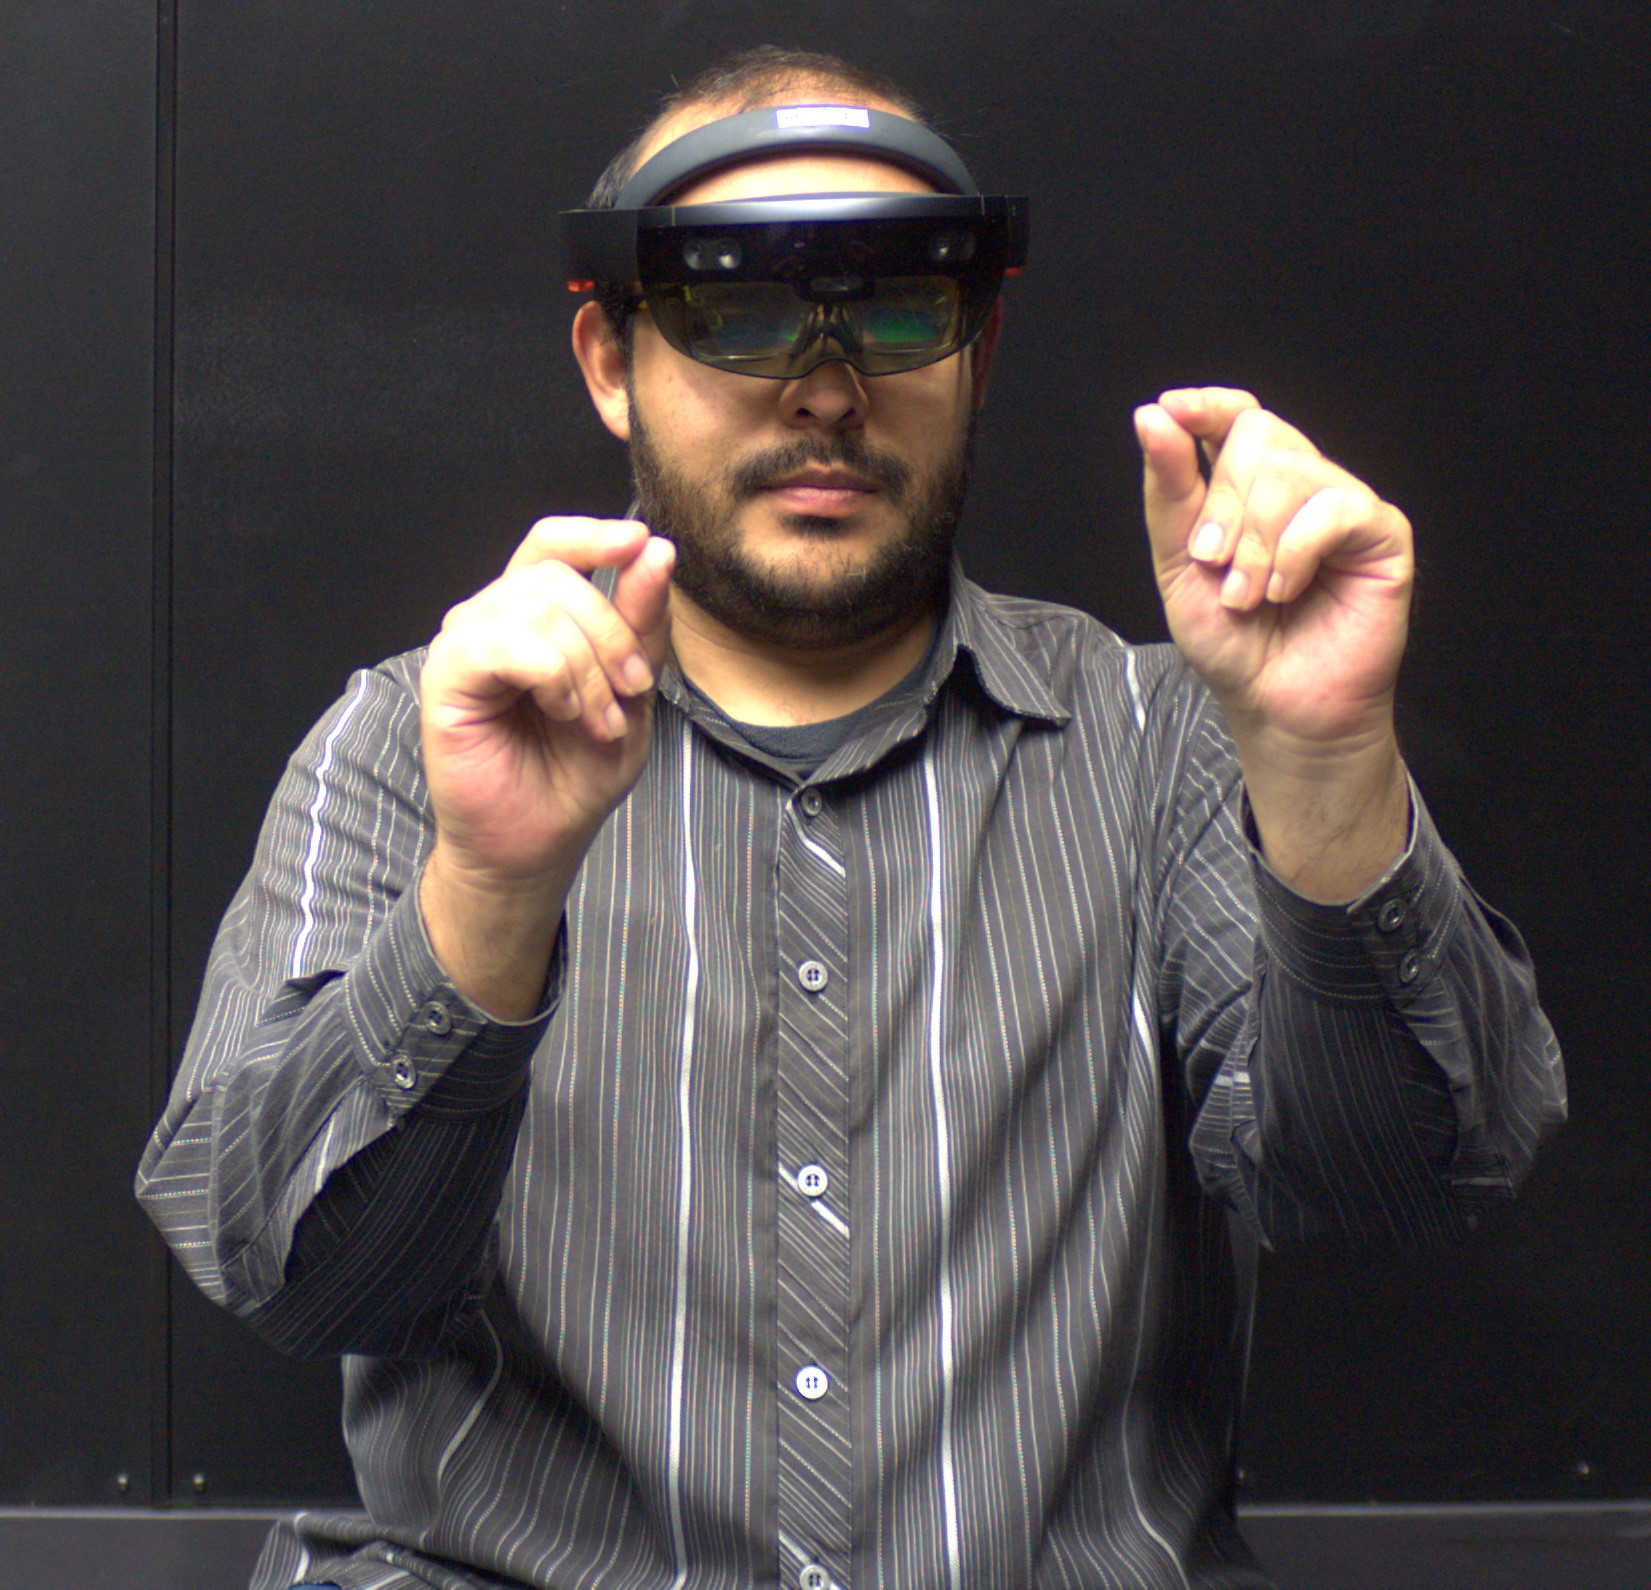
\includegraphics[alt={Figure 5.1b},width=0.5\textwidth,height=0.33\textheight]{figures/F5-1B.jpg}}
    \caption{Setups for Scenario 1 (using a smartphone, left) and Scenario 2 (using a HoloLens, right) \label{fig:5-1}}
\end{figure}

Both scenarios facilitated distinct modes of interaction, which were anticipated to influence the participants' thought processes and instinctive responses for each task. It was
hypothesised that:

\begin{itemize}
    \item Scenario 1 would prompt individuals to interact with the screen rather than the free hand.
    \item Scenario 2 would prompt more air gestures.
    \item Each scenario would converge to its own set of gestures rather than both converging to the same general set.
\end{itemize}

It is also important to note that at this point in the design of the software, it was not clear if \emph{WorkshopAR} was going to be implemented with full cross-platform compatibility in
mind, and it was therefore important to identify how users proposed gestures for the same task in different scenarios. If they diverged enough, it would be necessary to create two different
input systems. If there was some form of convergent set, that method could be used or expanded upon for the interaction proposal.

As noted in previous sections, \textcite{piumsomboon_2013} proposed a set of common tasks to perform in an \ac{AR} application. These tasks were classified into the selection, manipulation,
and transformation of digital objects. Nowadays these actions have become common and expected in any environment that requires 3D interactions, with the particularity that these tasks are
all related to single-user experiences. Based on ideas present in previous works \parencite{pinelle_2003,scoular_2020}, 14 tasks were identified, representing the most common activities
done in a collaborative activity and that could be supported by an \ac{AR} application. Three principles guided the final selection:

\begin{itemize}
    \item All or most members of the team are present in the same place. Remote collaboration was considered but not enforced or assumed.
    \item All members of the team have access to the same \ac{AR} application but not necessarily to the same platform nor do they have the same means of interaction.
    \item The context in which the collaboration is done can be varied (education, work, problem solving, etc.) with the objective of being applicable to any form of collaborative activity.
\end{itemize}

Table \ref{tab:5-1} shows the list of selected tasks divided into three distinct categories. The first category refers to asking another participant to pay attention to an element that is
part of the experience, often relating to its position or some describing characteristic. This action has been generalised as pointing and has also been separated into three similar tasks
with the purpose of analysing whereas the type of element being pointed at would change the behaviour of the participants. These tasks would ask to point at a digital construct created by
the app, at a physical or real object in the real space used for the augmented experience and at another person participating in the experience with them, another human user.

The second category refers to the actions the team could be doing simultaneously while interacting with the digital constructs provided by the application. Most tasks identified for this
category overlapped with common activities proposed in previous works, such as selecting, moving, and transforming objects. The collaborative context of this study would not change
substantially the way participants would approach any of those actions. To gather more pertinent data, only tasks related to sharing objects between team members were selected.

There is also a proposed distinction between a shared and a private space in which each member of the team can interact with different digital constructs, a concept similar to the ideas
discussed in works such as \textcite{reilly_2014,lebeck_2018}. The primary objective of this addition was to identify how the participants would visualise and interact with these spaces
and to investigate whether the different scenarios would influence their ideas and responses.

The final category are elements common to team management \parencite{zigurs_2006}, those that could benefit from \ac{AR} augmentation, or at the very least, be compatible within an \ac{AR}
setting. This assumption was particularly relevant given the decision to maintain synchronous team interactions within the same physical space. This category also considers actions done by
an individual managing an activity for several groups at the same time, like a teacher or a coach guiding the experience.

\begin{table}[]
\caption{Proposed Collaboration Tasks in \ac{AR}}
\begin{tabularx}{\textwidth}{@{}ccX@{}}
\textbf{Category}                    & \multicolumn{2}{c}{\textbf{Task}}                          \\ \midrule
\multirow{3}{*}{Pointing}            & 1  & Pointing at a digital object                          \\ 
                                     & 2  & Pointing at a physical object or space                \\ 
                                     & 3  & Pointing at a person                                  \\ \midrule
\multirow{5}{*}{Shared Manipulation} & 4  & Hold an object                                        \\ 
                                     & 5  & Share an object with someone else                     \\ 
                                     & 6  & Take an object into a private space                   \\ 
                                     & 7  & Undo an action                                        \\ 
                                     & 8  & Take an object out of the private space               \\ \midrule
\multirow{6}{*}{Team Management}     & 9  & Vote for an option in a menu                          \\ 
                                     & 10 & Vote for an option in a collection of digital objects \\ 
                                     & 11 & Ask for the attention of others                       \\ 
                                     & 12 & Pause current participation                           \\ 
                                     & 13 & Give someone the turn to speak                        \\ 
                                     & 14 & Ask for the attention of all the teams                \\ \bottomrule
\end{tabularx}
\label{tab:5-1}
\end{table}

A simple application was built to visualise animations representing each task. This also allowed a more realistic sense of how the activities would be carried out using the assigned device.
The participants were able to only see the animations but not interact with the digital constructs in any way. They could also repeat the animation any number of times and move between the
animations of different tasks at will. The application worked in the exact same way in both scenarios. Figure \ref{fig:5-2} shows some examples of what the participants could see in the
application.

\begin{figure}
    \centering{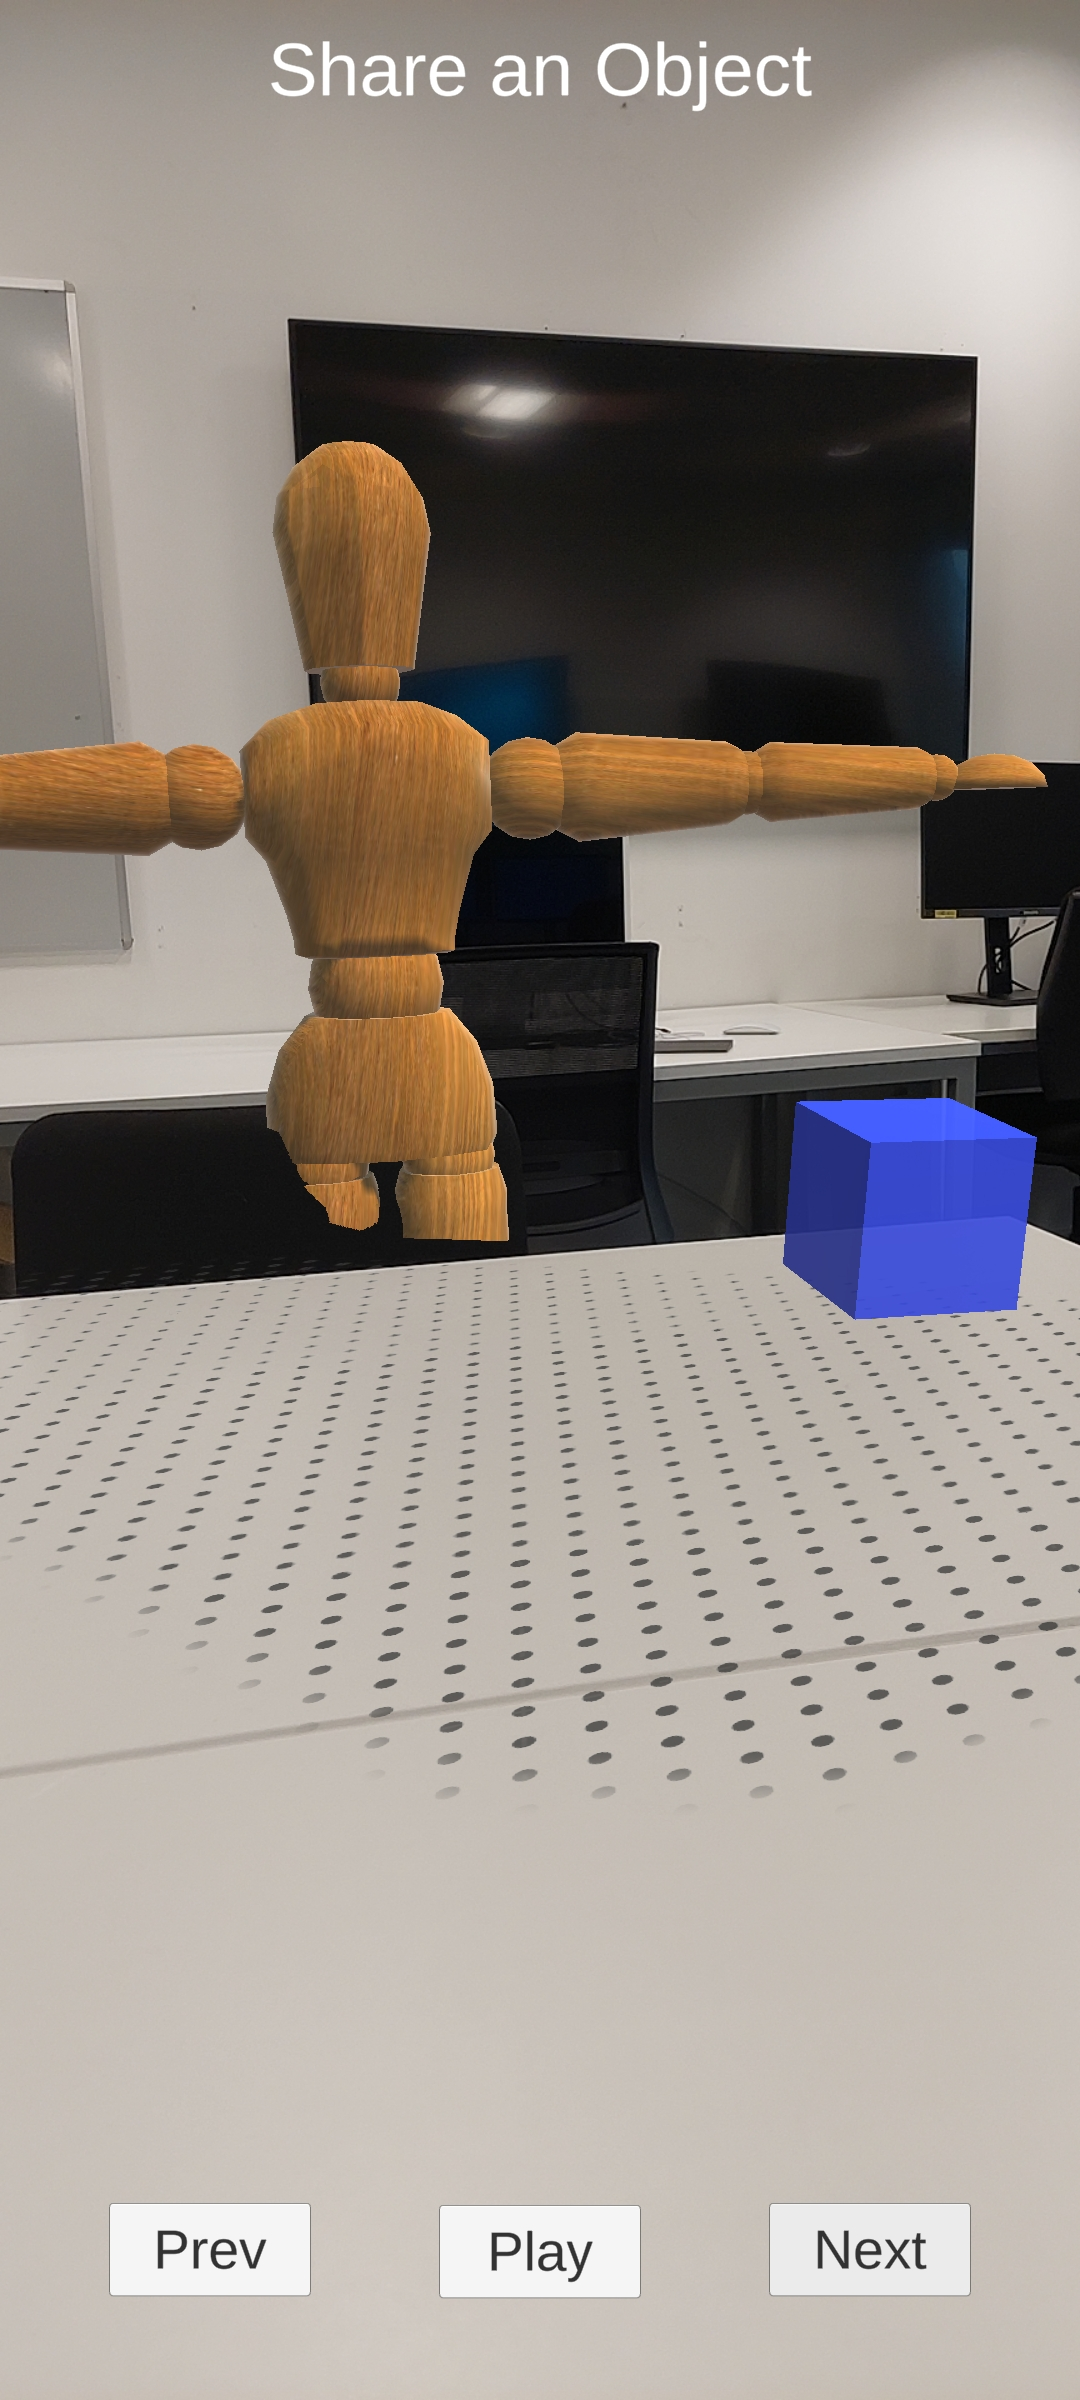
\includegraphics[alt={Figure 5.2a},width=0.49\textwidth,height=0.6\textheight]{figures/F5-2A.jpg}}
    \centering{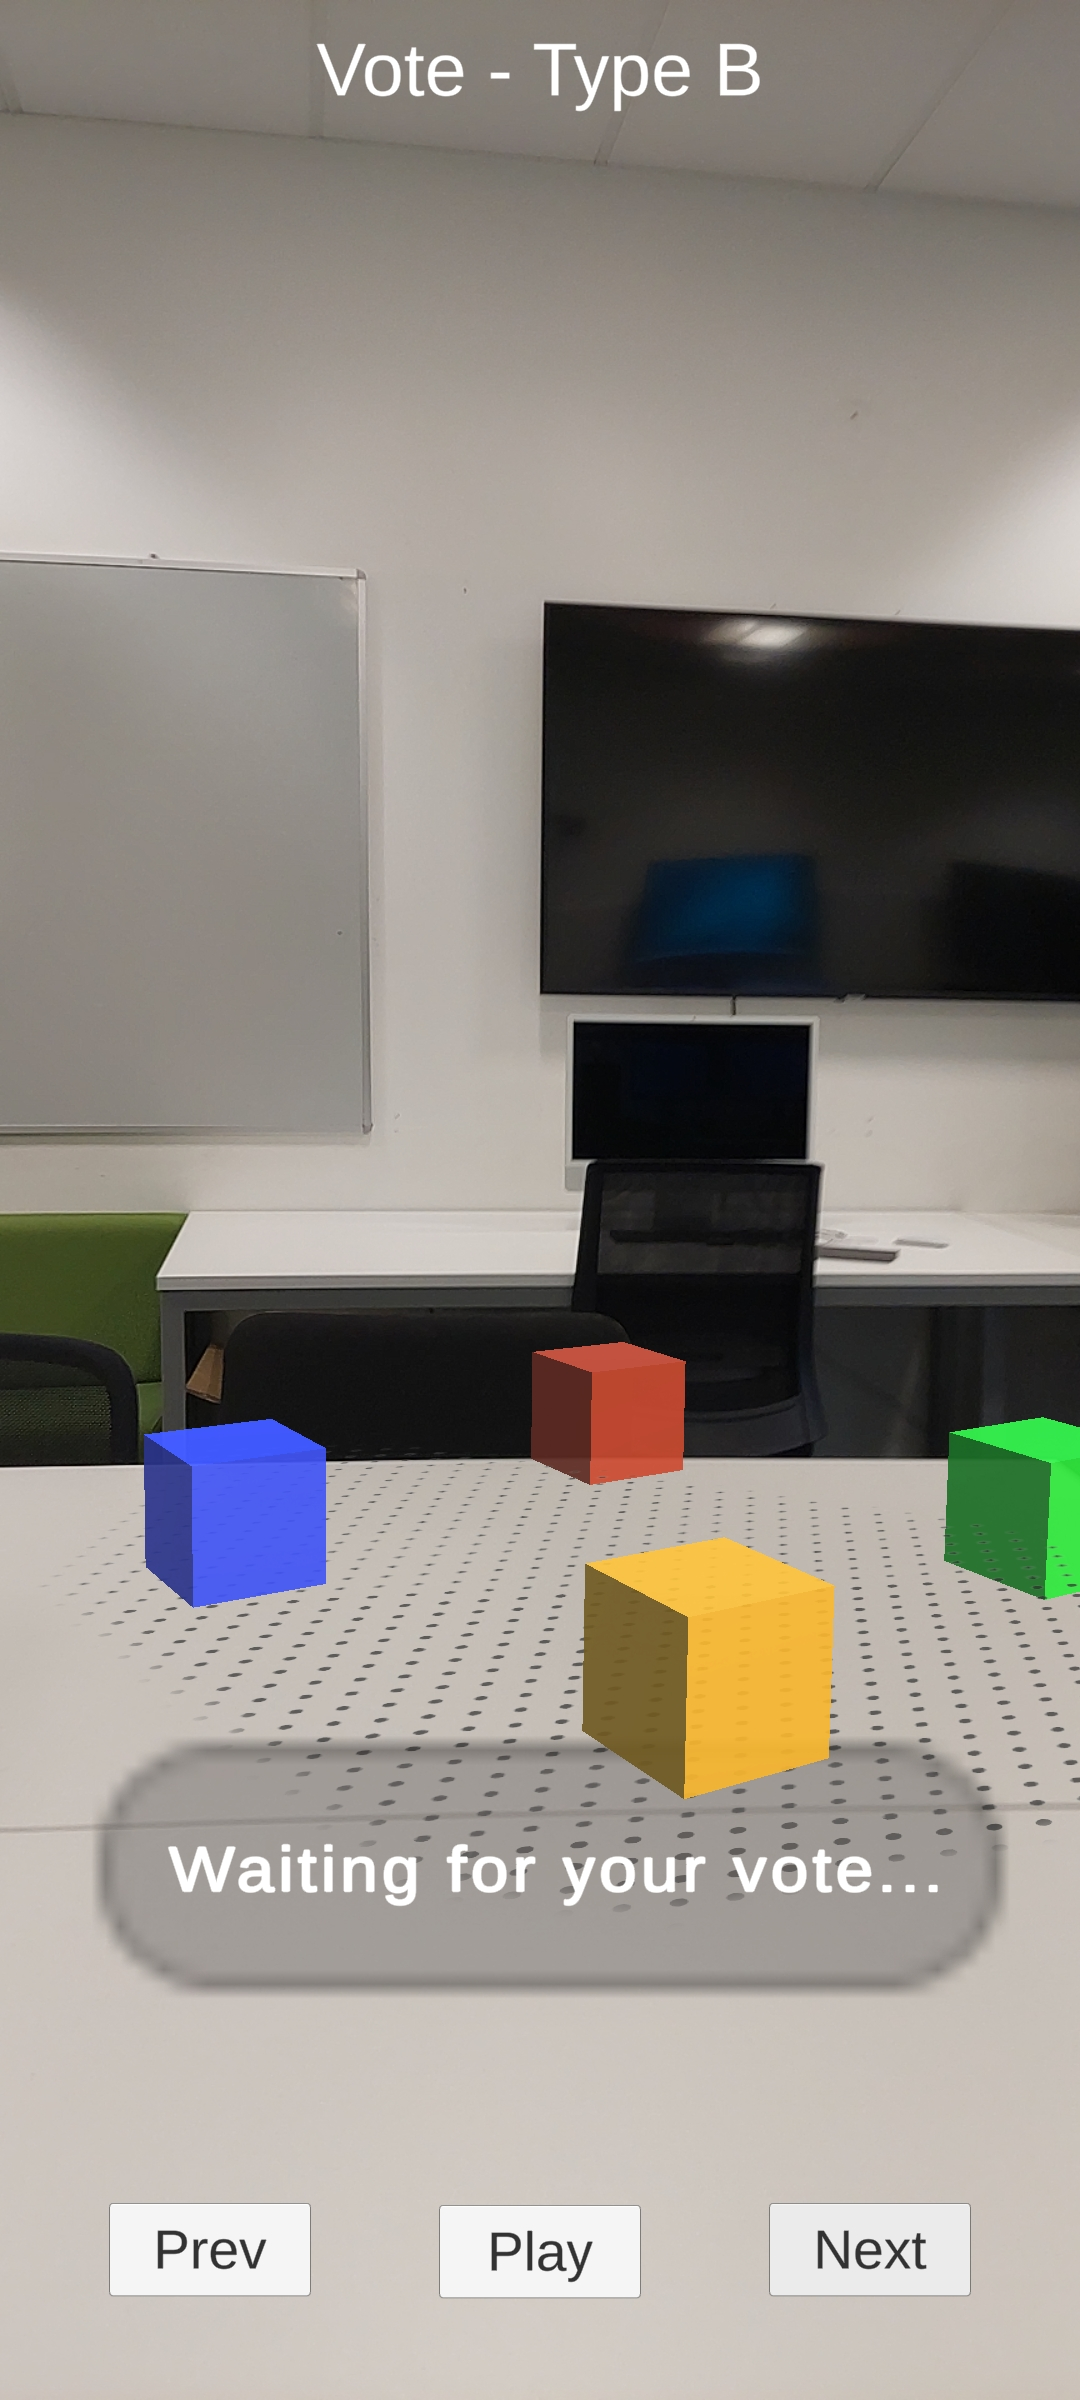
\includegraphics[alt={Figure 5.2b},width=0.5\textwidth,height=0.6\textheight]{figures/F5-2B.jpg}}
    \caption{Example Views of the Share an Object (left) and Vote with Objects (right) Tasks \label{fig:5-2}}
\end{figure}

Each participant was assigned one of the two scenarios (smartphone or HoloLens), alternating between the options to ensure a balanced distribution. Each participant was given a brief
introduction and an explanation of what was expected of them by the researcher. Additionally, they were given a brief tutorial of the basic usage of each setup. Special emphasis was placed
on showing how they could put their hands in front of the camera to simulate an interaction, but they were still reminded that they could do whatever they thought would be most natural or
straightforward to achieve the action presented to them.

All participants would then proceed through each task performing any number of interactions that would come to mind and trying to verbalise their thought processes and logic. Participants
could propose any number of interactions. If none of the proposed interactions were air gestures, the researcher would remind them of that possibility. Tasks were always given to the
participants in the same order to simplify the process of explaining the task context and managing the flow of the session.

The specific emphasis on air gestures is due to their strong association with AR technology, which often uses image recognition techniques to track the users' hands and use them for
interactions in a more natural and intuitive way \parencite{lu_2022,gavgiotaki_2023}. It was also theorised that participants would not necessarily be familiar with either the technology
or those common interaction metaphors, so it was decided that an explicit mention of air gestures after the first round of proposals made by the users would help in the generation of ideas
and would also help gather data concerning the hypotheses built for each scenario.

To capture the raw data, all sessions were recorded with a video camera for analysis. The recordings took place over several weeks and in different spaces, sometimes with the participants
seated and some other times standing, but always with the same equipment, the same test software, and following the same procedure.

Another important decision was to gather the data of each participant individually. Although the interactions were associated with group activities, there was no need, nor did the process
gain anything by simulating the full teamwork experience. On the other hand, if the process would have been more complex, it would have been necessary to coordinate several participants in
time and space, and the mock-up software would have also grown in complexity to accommodate several users. It was deemed as an unnecessary development. The procedure clearly explained to
the participants that the activity meant to simulate a teamwork scenario with other humans, and some measures were taken to add to the animations presented by the software simple
representations of other users to give the participants a visual idea of the scenario presented to them (See Figure \ref{fig:5-2}, left).

Each of the recordings underwent analysis to create a transcript of all the participants' comments and ideas, as well as to identify common thoughts, problems, and solutions. Video footage
of each session was processed to compile a library of all the gestures performed for each task. Each individual performance of a gesture was given a score from 1 to 3, with the highest
score given to the first gesture proposed by a participant. If a participant proposed two or more gestures or proposed a gesture after being prompted by the researcher, those gestures were
given a lower score. This meant that gestures with a higher score were performed the most and could be interpreted as the most natural or intuitive reaction for most of the participants.
All gestures after the third proposal received a score of 1.

A total of 478 gestures were proposed for all tasks. Although each task clearly converged to a specific set of gestures, agreement in general was low. For each task, agreement was
calculated using equation \ref{eq:5-1} \parencite{wobbrock_2005}.

\begin{equation}
    A = \sum_{N}^{}\Big(\frac{P_{s}}{P_{t}}\Big)^{2} \label{eq:5-1}
\end{equation}

In this equation, Pt is the total number of gestures performed for a task, and Ps is the number of times a distinct gesture was performed by different participants. This gives a value of
agreement for each task up to 1, which would mean that every participant proposed the same gesture for the task, while a value closer to 0 means that every participant proposed a different
gesture. Figure \ref{fig:5-3} shows the level of agreement reached for each task and in each scenario in descending order.

\begin{figure}
    \centering{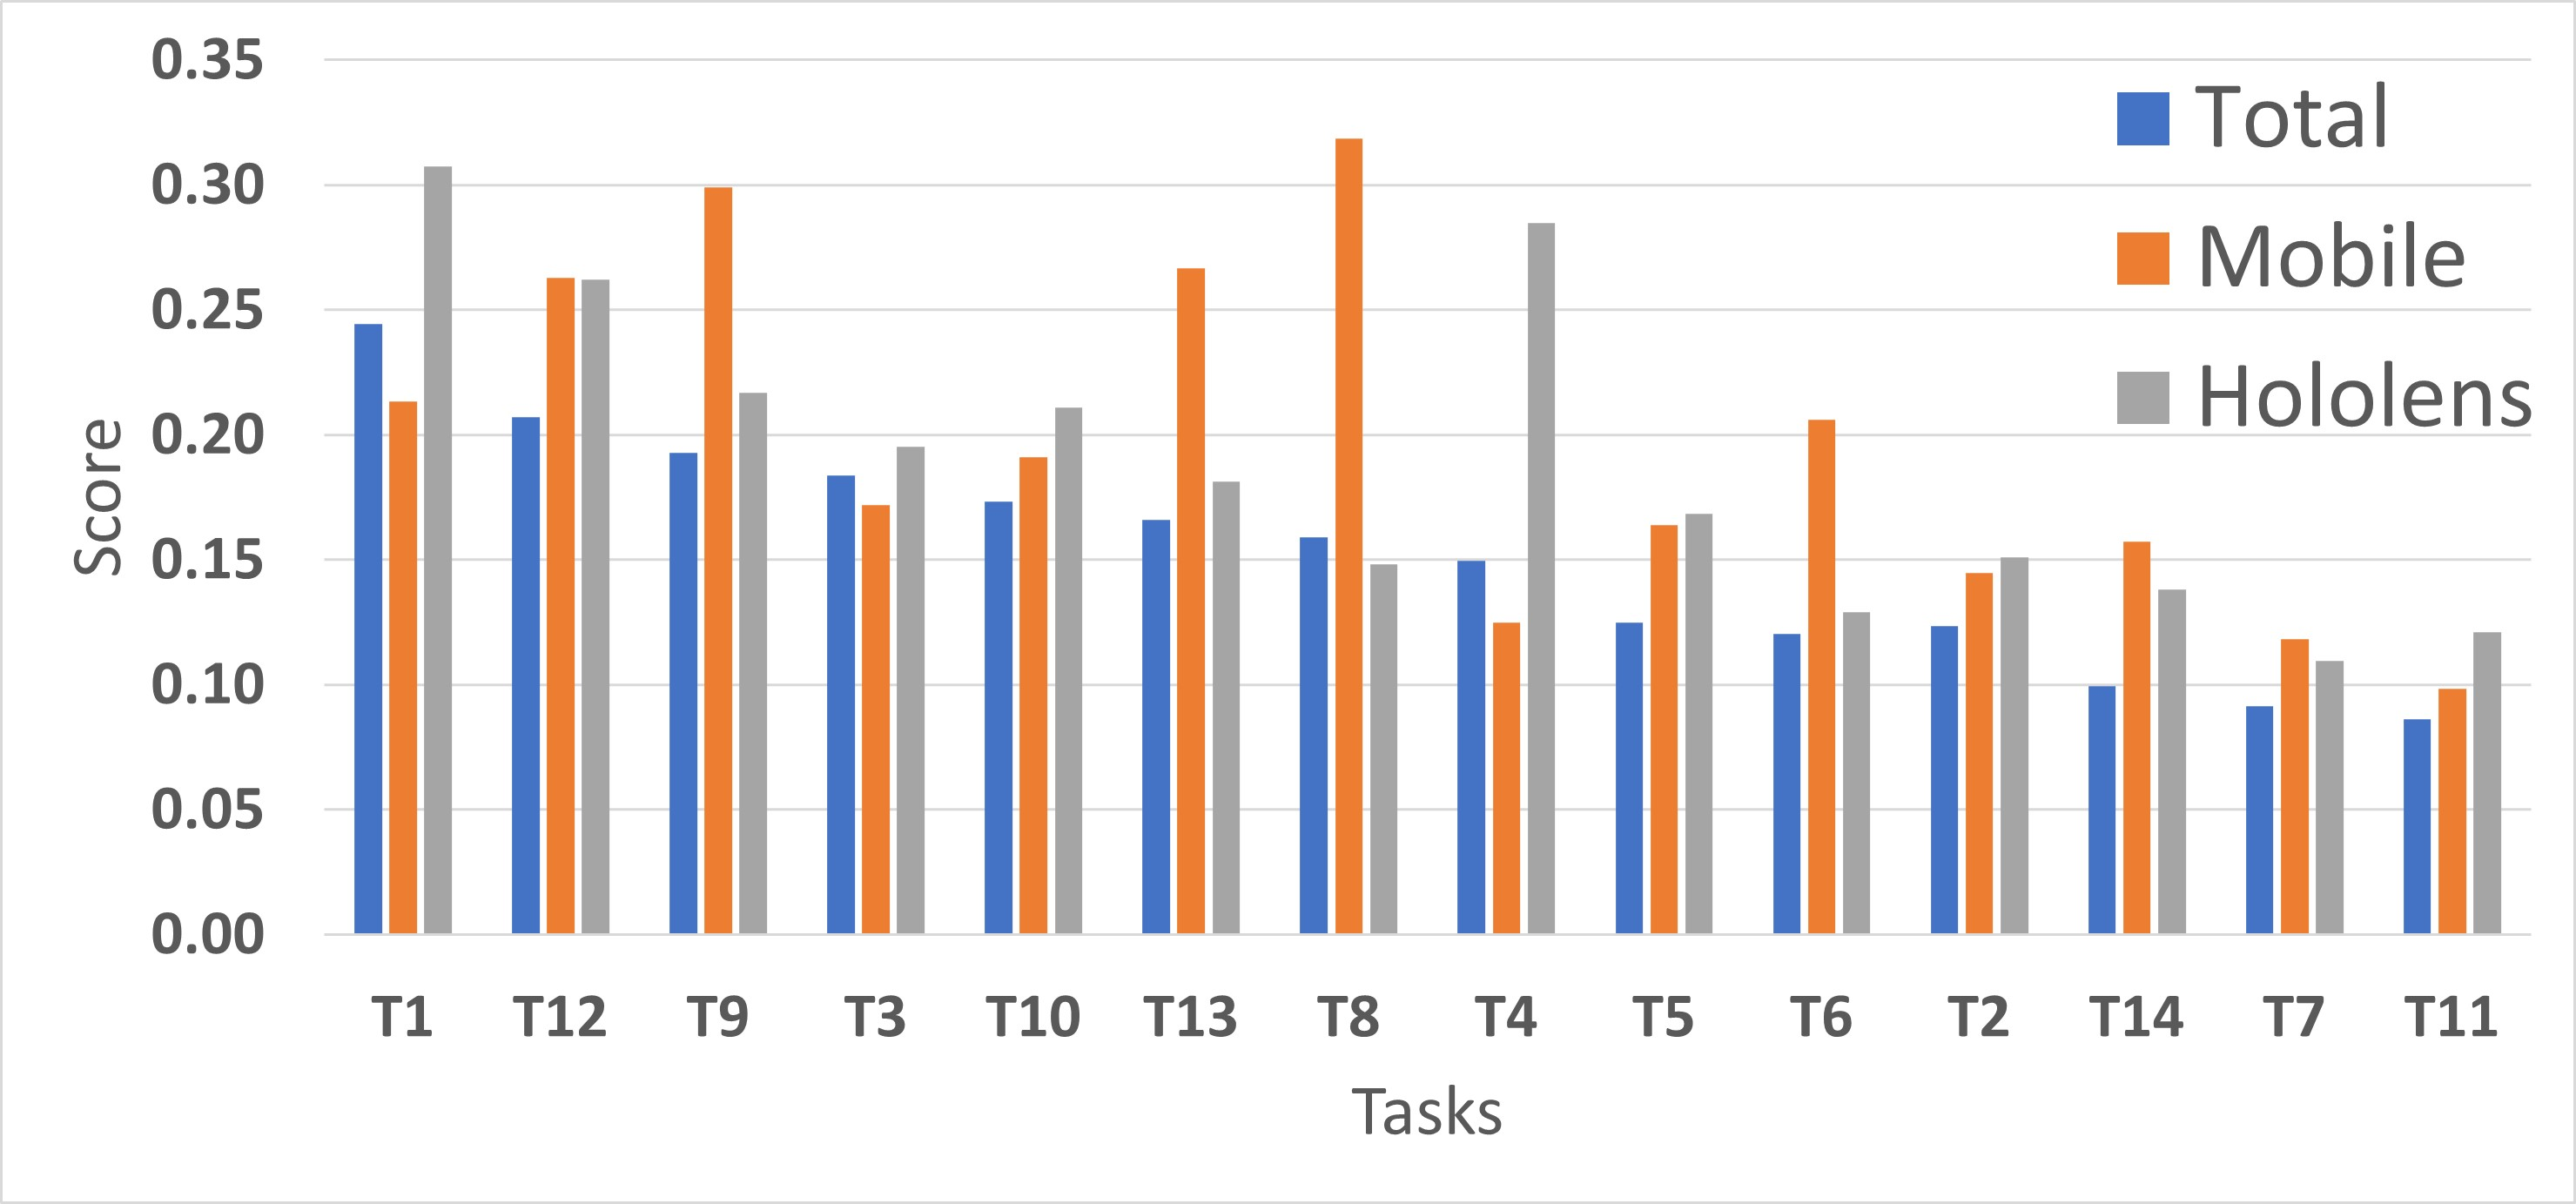
\includegraphics[alt={Figure 5.3},width=0.99\textwidth]{figures/F5-3.jpg}}
    \caption{Total Agreement Scores for Each Task, Separated by Scenario \label{fig:5-3}}
\end{figure}

Overall, tasks 1, 12 and 9 had the highest agreement, corresponding to pointing at an object, pausing your participation, and voting for an option on a menu. Although these tasks are the
most prominent examples, all of them behaved in the same manner, with most of the participants agreeing on one or two gestures, but the rest proposing a very granular or unique set,
generally bringing down the agreement score significantly for all tasks. It is also important to note that the agreement score for both scenarios aggregated is a bit lower than when
separated by scenario. Tasks 8, 9 and 13 had a better score in the mobile scenario, mainly because they were strongly associated with touch actions on the screen and most participants
converged to such interactions. On the other hand, the HoloLens scenario had better scores for tasks 1 and 4 (point to and hold and object), probably because the tasks suggested obvious or
natural hand movements to which most of the participants converged.

\subsubsection{Proposed Interaction Gestures \label{sec:5-1-1-2}}

Based on all the data provided by the participants, a library of 39 gestures was selected as the final user-driven selection. These gestures cover 56\% of the total proposals and the set of
each task represents between 50\% and 70\% of them. The following section will show the final agreement score for all the unique gestures identified in each task, as well a visual example
of the gestures selected for the final collection, the one that exemplifies best the ideas to which the users converged at. Access to video captures for all the gestures identified in each
task is provided in Appendix \ref{appendix:b}.

Tasks 1, 2 and 3 are related to pointing elements of the environment to the team. These tasks were the ones with the highest agreement scores in both scenarios. Participants defaulted to
pointing with one or two fingers towards the camera in the general direction of the digital object or trying to superpose the gesture over the object. Figure \ref{fig:5-4} shows the
agreement score for the 11 unique gestures identified for the task.

\begin{figure}
    \centering{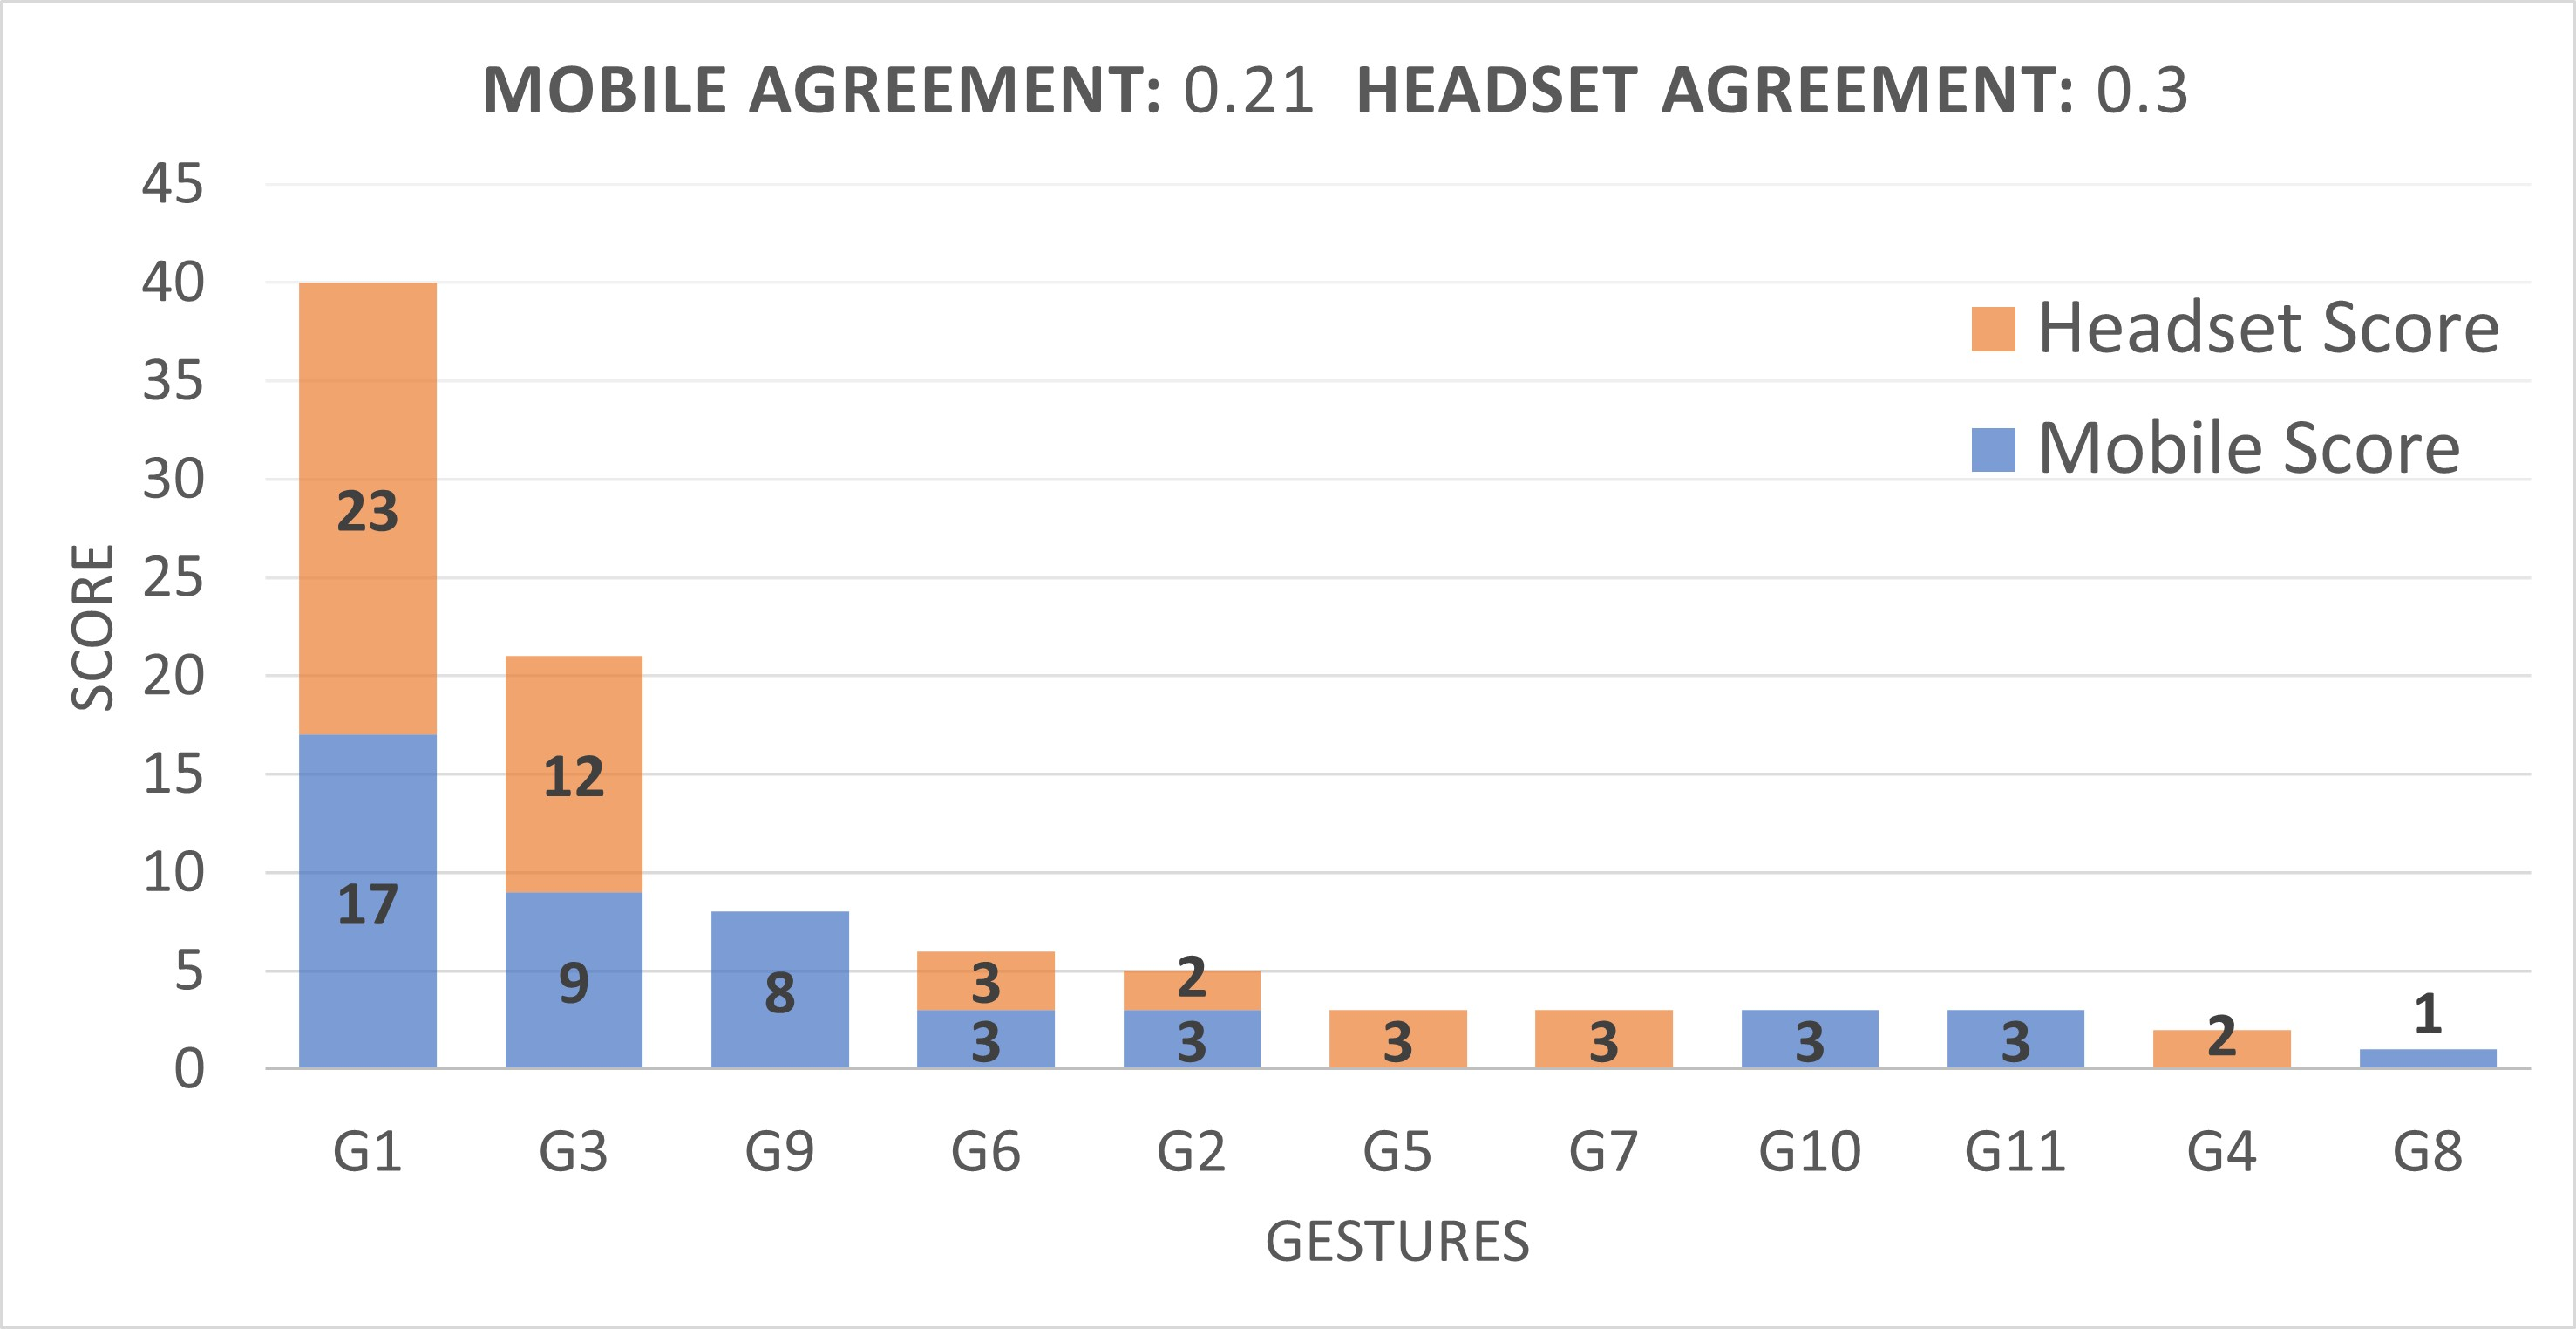
\includegraphics[alt={Figure 5.4},width=0.99\textwidth]{figures/F5-4.jpg}}
    \caption{Agreement scores for unique gestures in Task 1 \label{fig:5-4}}
\end{figure}

The selected gestures involved pointing directly to the object with one or two fingers, with a stronger tendency for this gesture in the headset scenario, while mobile users defaulted more
to tapping motions in the screen. The most important reasoning given by the users for the tapping behaviour was that the motion was \emph{natural} or \emph{common}, especially for a touch
screen. In scenario 2 some users also mentioned the naturality of the tapping motion comparing it to touching a screen, highlighting the influence of previous knowledge when translating
the actions to a scenario that is similar or somewhat familiar. The tapping motion also included stronger deviations of the gesture, like using the whole hand or exaggerating the pointing
motion of the object to make clear the intended selection and to eliminate ambiguity in the selection, a concern mentioned by some users.

A variation proposed consisted of grabbing or holding the object to signify to others that \emph{this object here that I am shaking is the one I am talking about}, to use the words of one
user. The mechanics of holding the object varied a lot between users, sometimes using one hand or both, and with or without movement involved after the grabbing motion.

It is also important to mention that the task was described to the users as \emph{pointing} to an object, which could have predisposed the users to a particular set of gestures. The task
was described as such to convey the idea that the action was done for the benefit of another user, and that the main objective was to highlight the object to another person, not only to
select the object. Nonetheless, a more neutral term could have been used, like \emph{show}, \emph{mention} or \emph{indicate}. Figure \ref{fig:5-5} shows an example of the selected gestures
for task 1, Figure \ref{fig:5-5} (left) depicts Task 1, Gesture 1 (T1G1) : Pointing at the object with the index finger, while Figure \ref{fig:5-5} (right) shows T1G3: Tapping the object with
the index finger.

\begin{figure}
    \centering{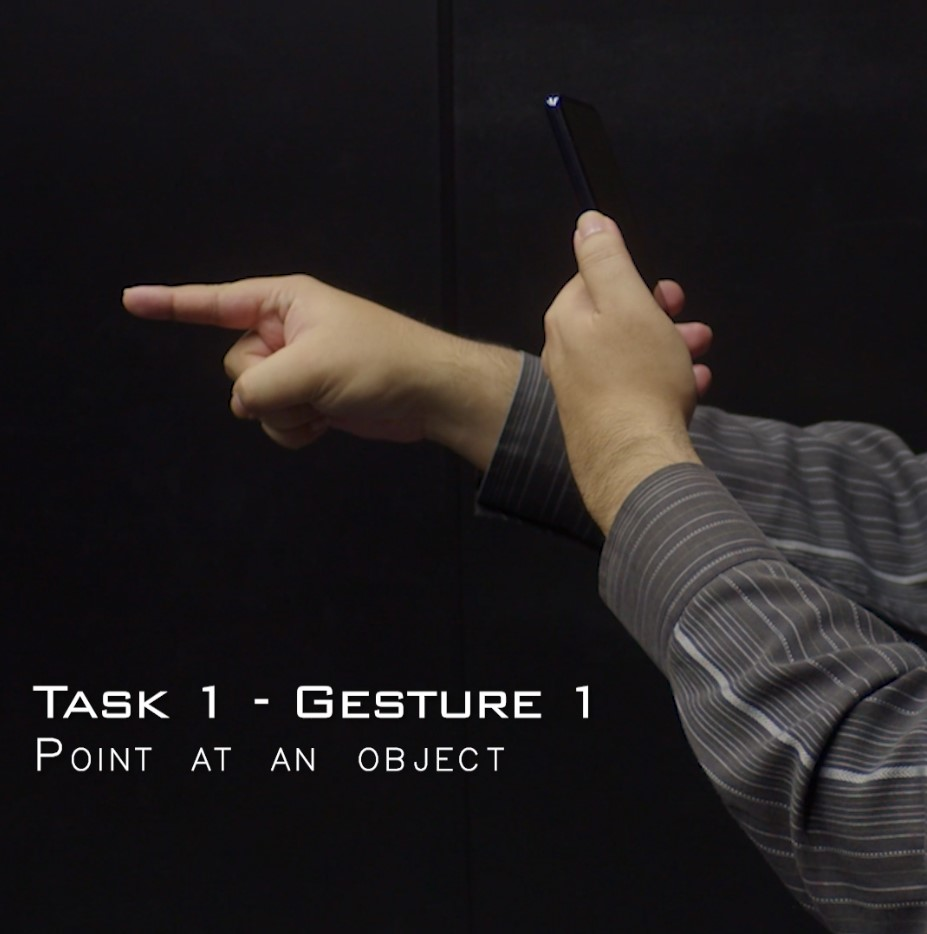
\includegraphics[alt={Figure 5.5a},width=0.49\textwidth,height=0.33\textheight]{figures/F5-5A.jpg}}
    \centering{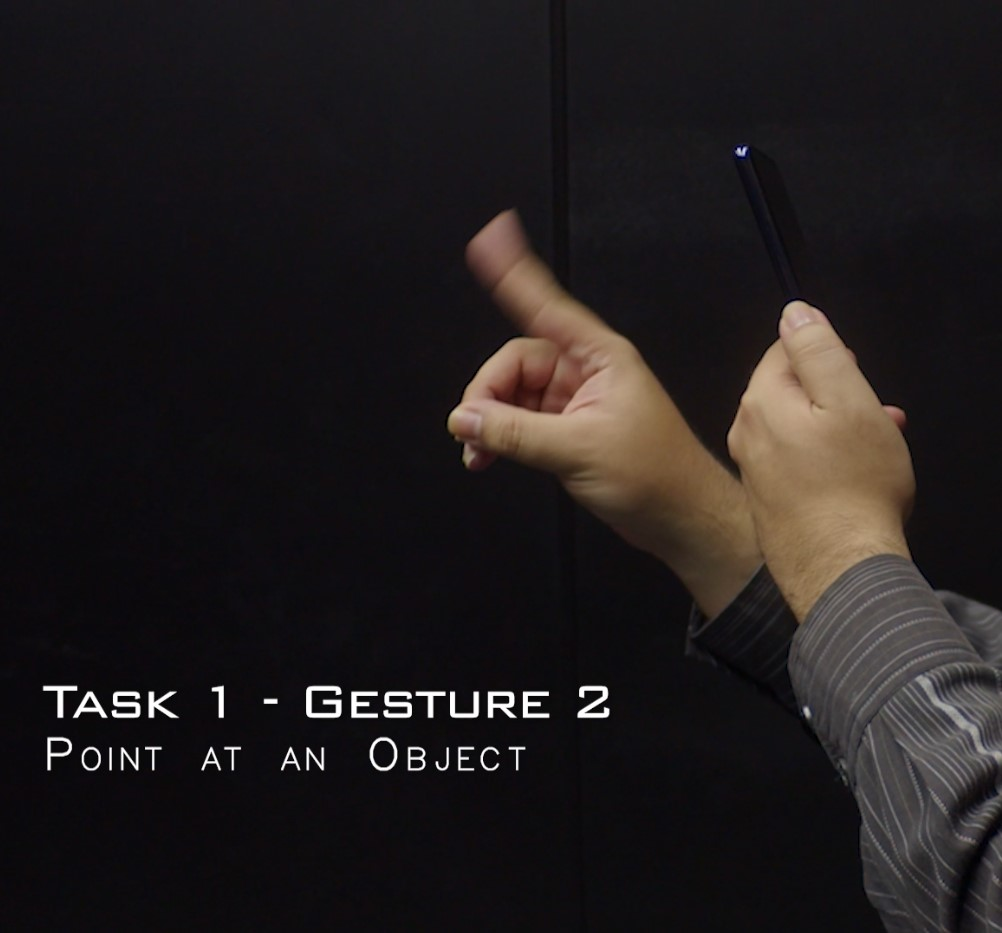
\includegraphics[alt={Figure 5.5b},width=0.5\textwidth,height=0.33\textheight]{figures/F5-5B.jpg}}
    \caption{Point at an object - Pointing  Index (left) and Tapping Motion (right) \label{fig:5-5}}
\end{figure}

Task 2 yielded very similar results. Participants used more descriptors or directions related to real-world elements. Phrases such as \emph{the one next to the chair} or \emph{the one next to your hand}
were common, but these comments were always accompanied by the same pointing gesture. Figure \ref{fig:5-6} shows the agreement score for the 15 unique gestures identified for Task 2.

\begin{figure}
    \centering{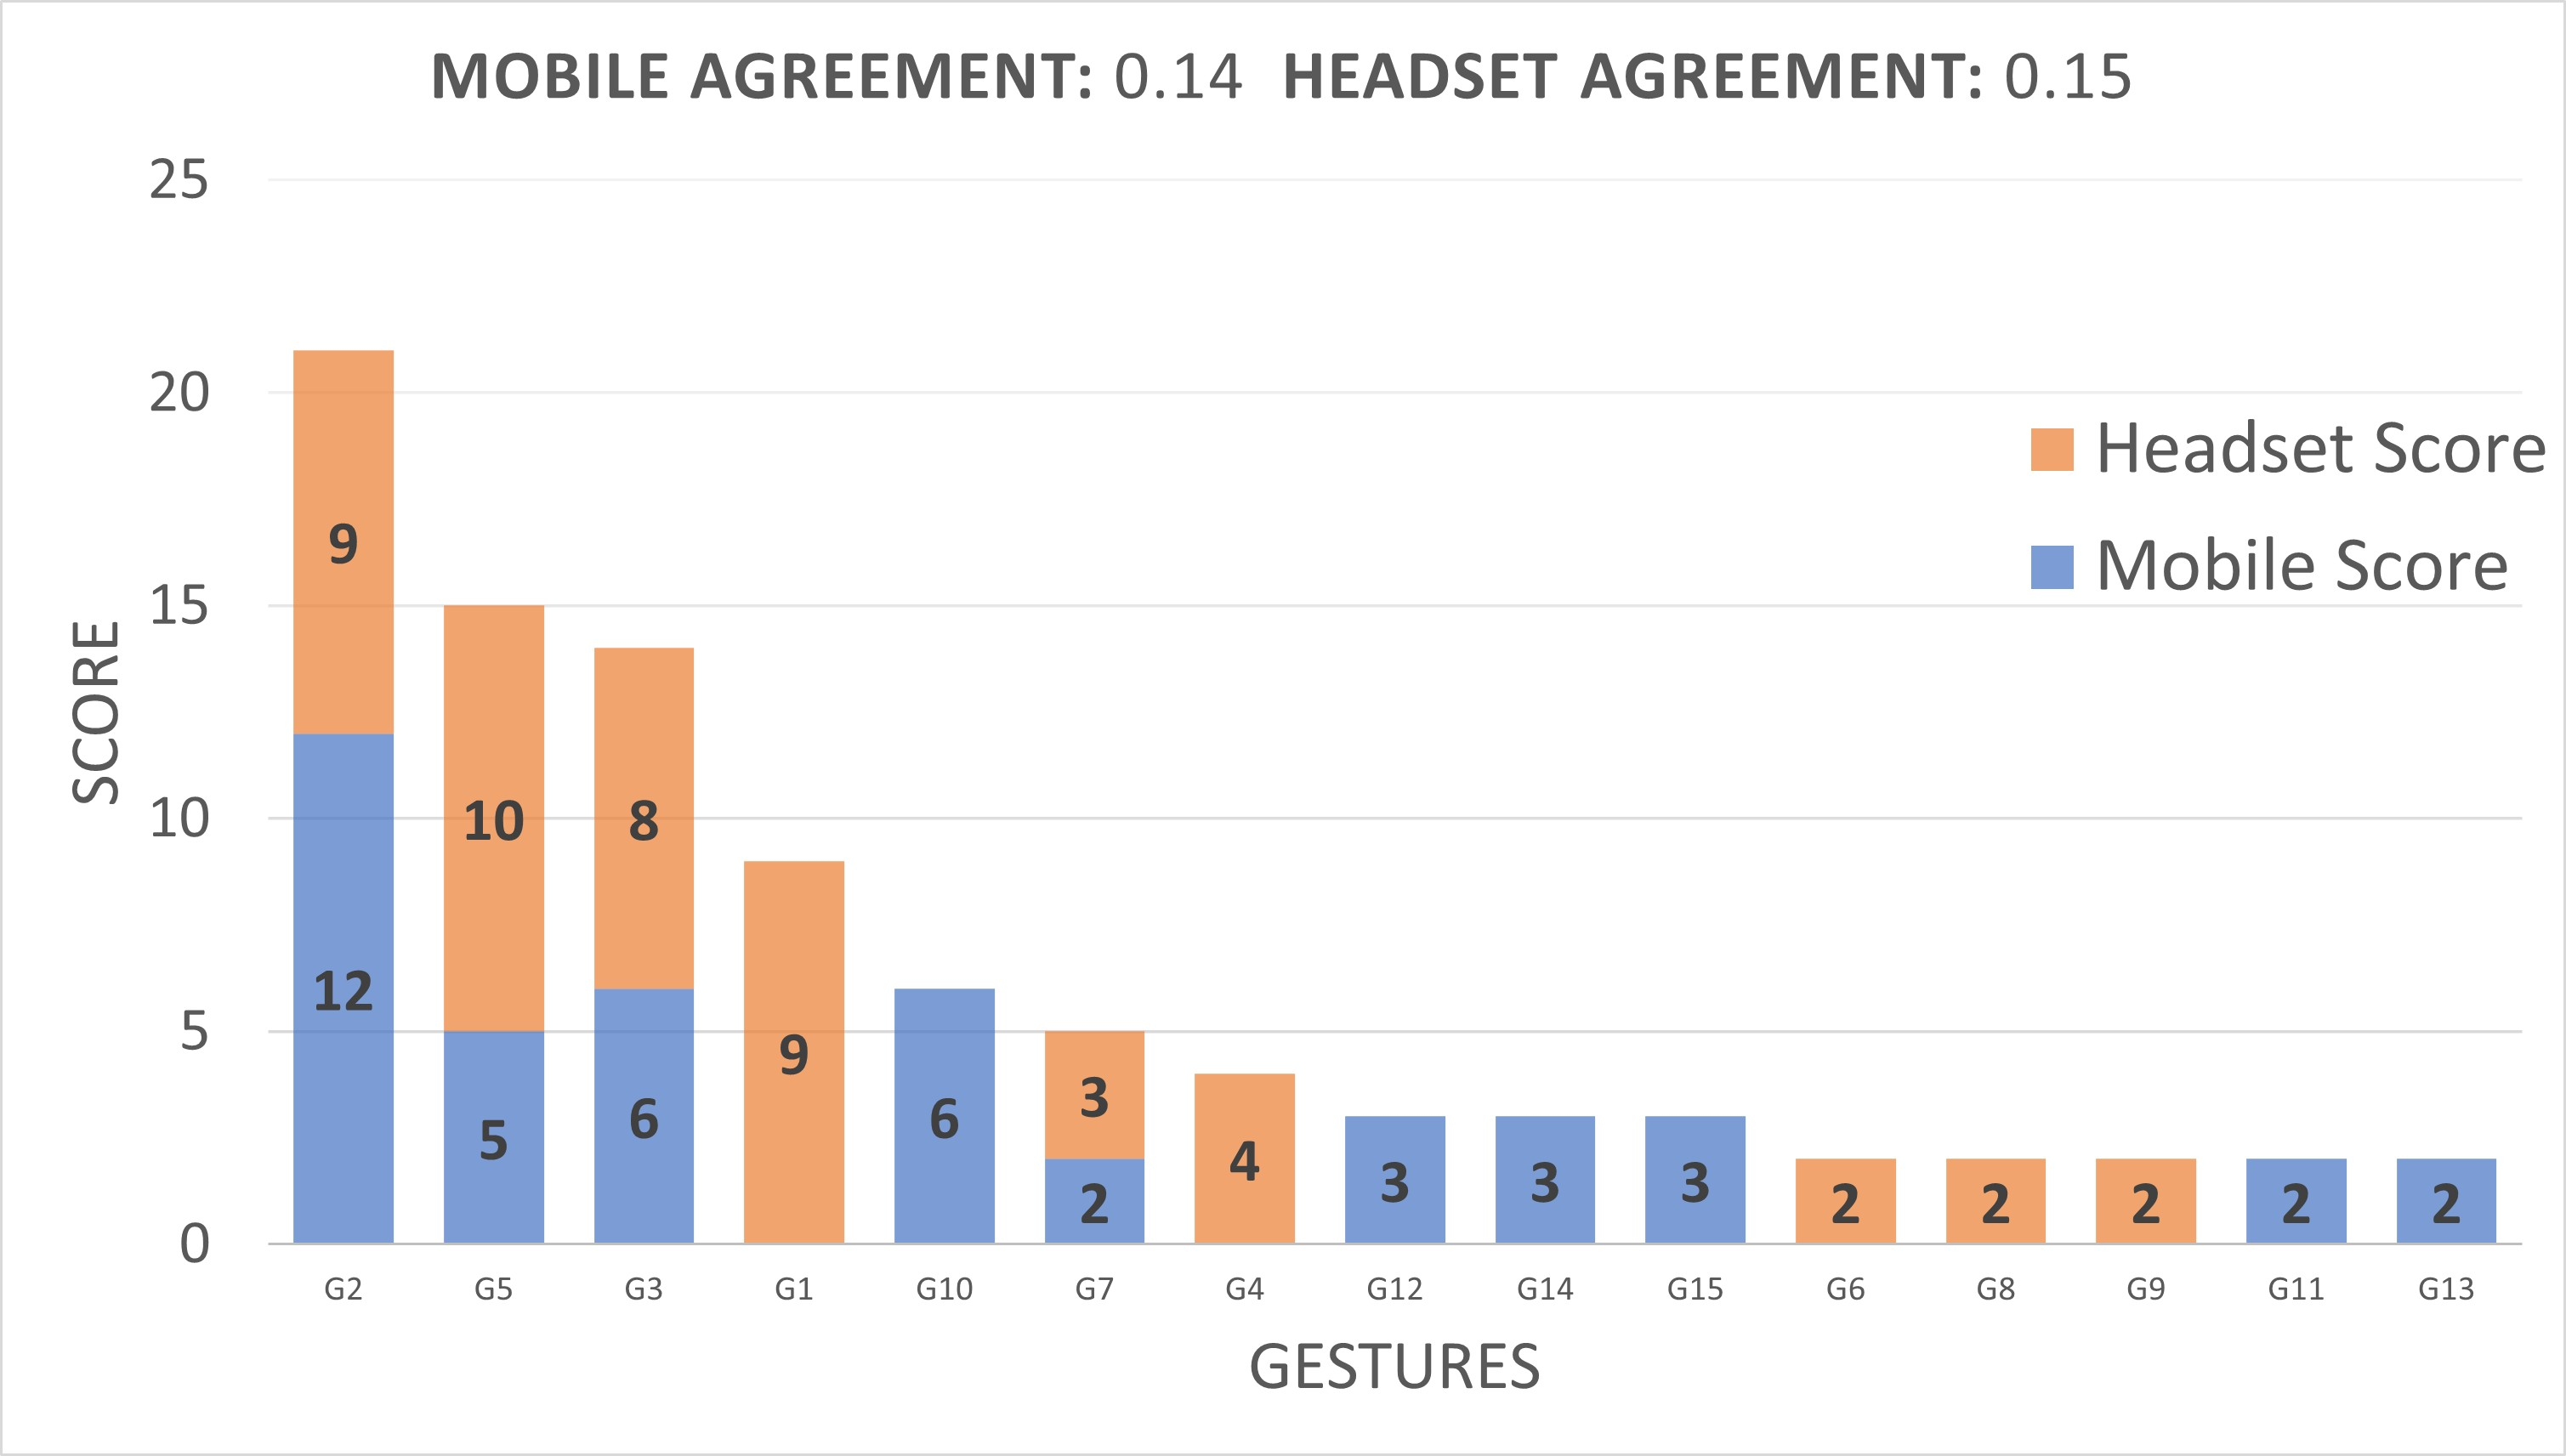
\includegraphics[alt={Figure 5.6},width=0.99\textwidth]{figures/F5-6.jpg}}
    \caption{Agreement scores for unique gestures in Task 2 \label{fig:5-6}}
\end{figure}

A significant number of users defaulted to use the whole hand for the pointing gesture, but it was not possible to identify a reason for such a difference in comparison to Task 1. Figure \ref{fig:5-7}
shows an example of this gesture. Another common proposal was to draw some figure to enclose the point in space being pointed at, like a circle, an X or some movement of the fingers.

\begin{figure}
    \centering{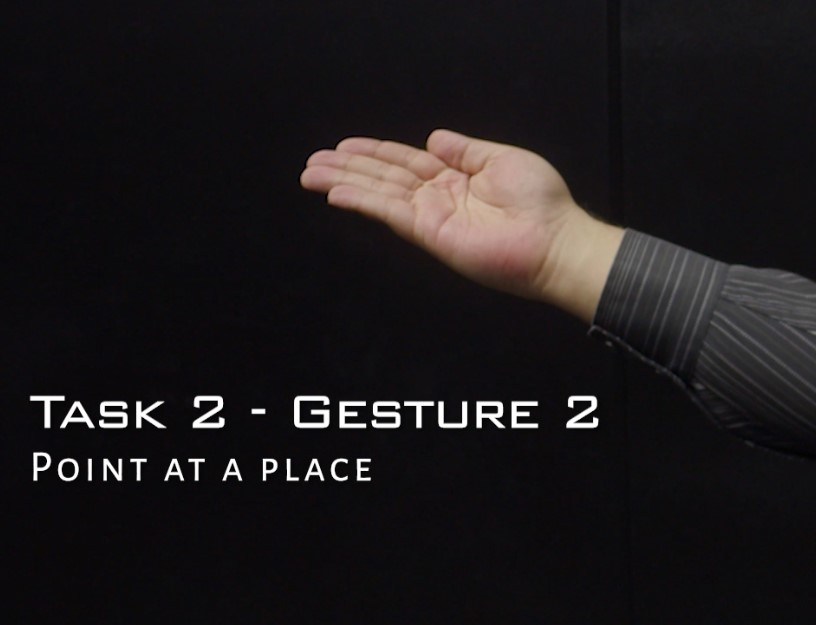
\includegraphics[alt={Figure 5.7},scale=0.5]{figures/F5-7.jpg}}
    \caption{Point at a place - Extended hand gesture \label{fig:5-7}}
\end{figure}

A similar situation was present in Task 3 when pointing to a person. In this scenario, the extended hand gesture was explicitly explained by the participants, who expressed reservations
about pointing at someone else with a finger, considering it disrespectful. They preferred to point using the entire hand with the same gesture shown in Figure \ref{fig:5-7} or by tapping
on the screen. Otherwise, the same tendencies shown in the previous two tasks were also present in here. Figure \ref{fig:5-8}  shows the agreement score for all the 13 unique gestures
identified for Task 3.

\begin{figure}
    \centering{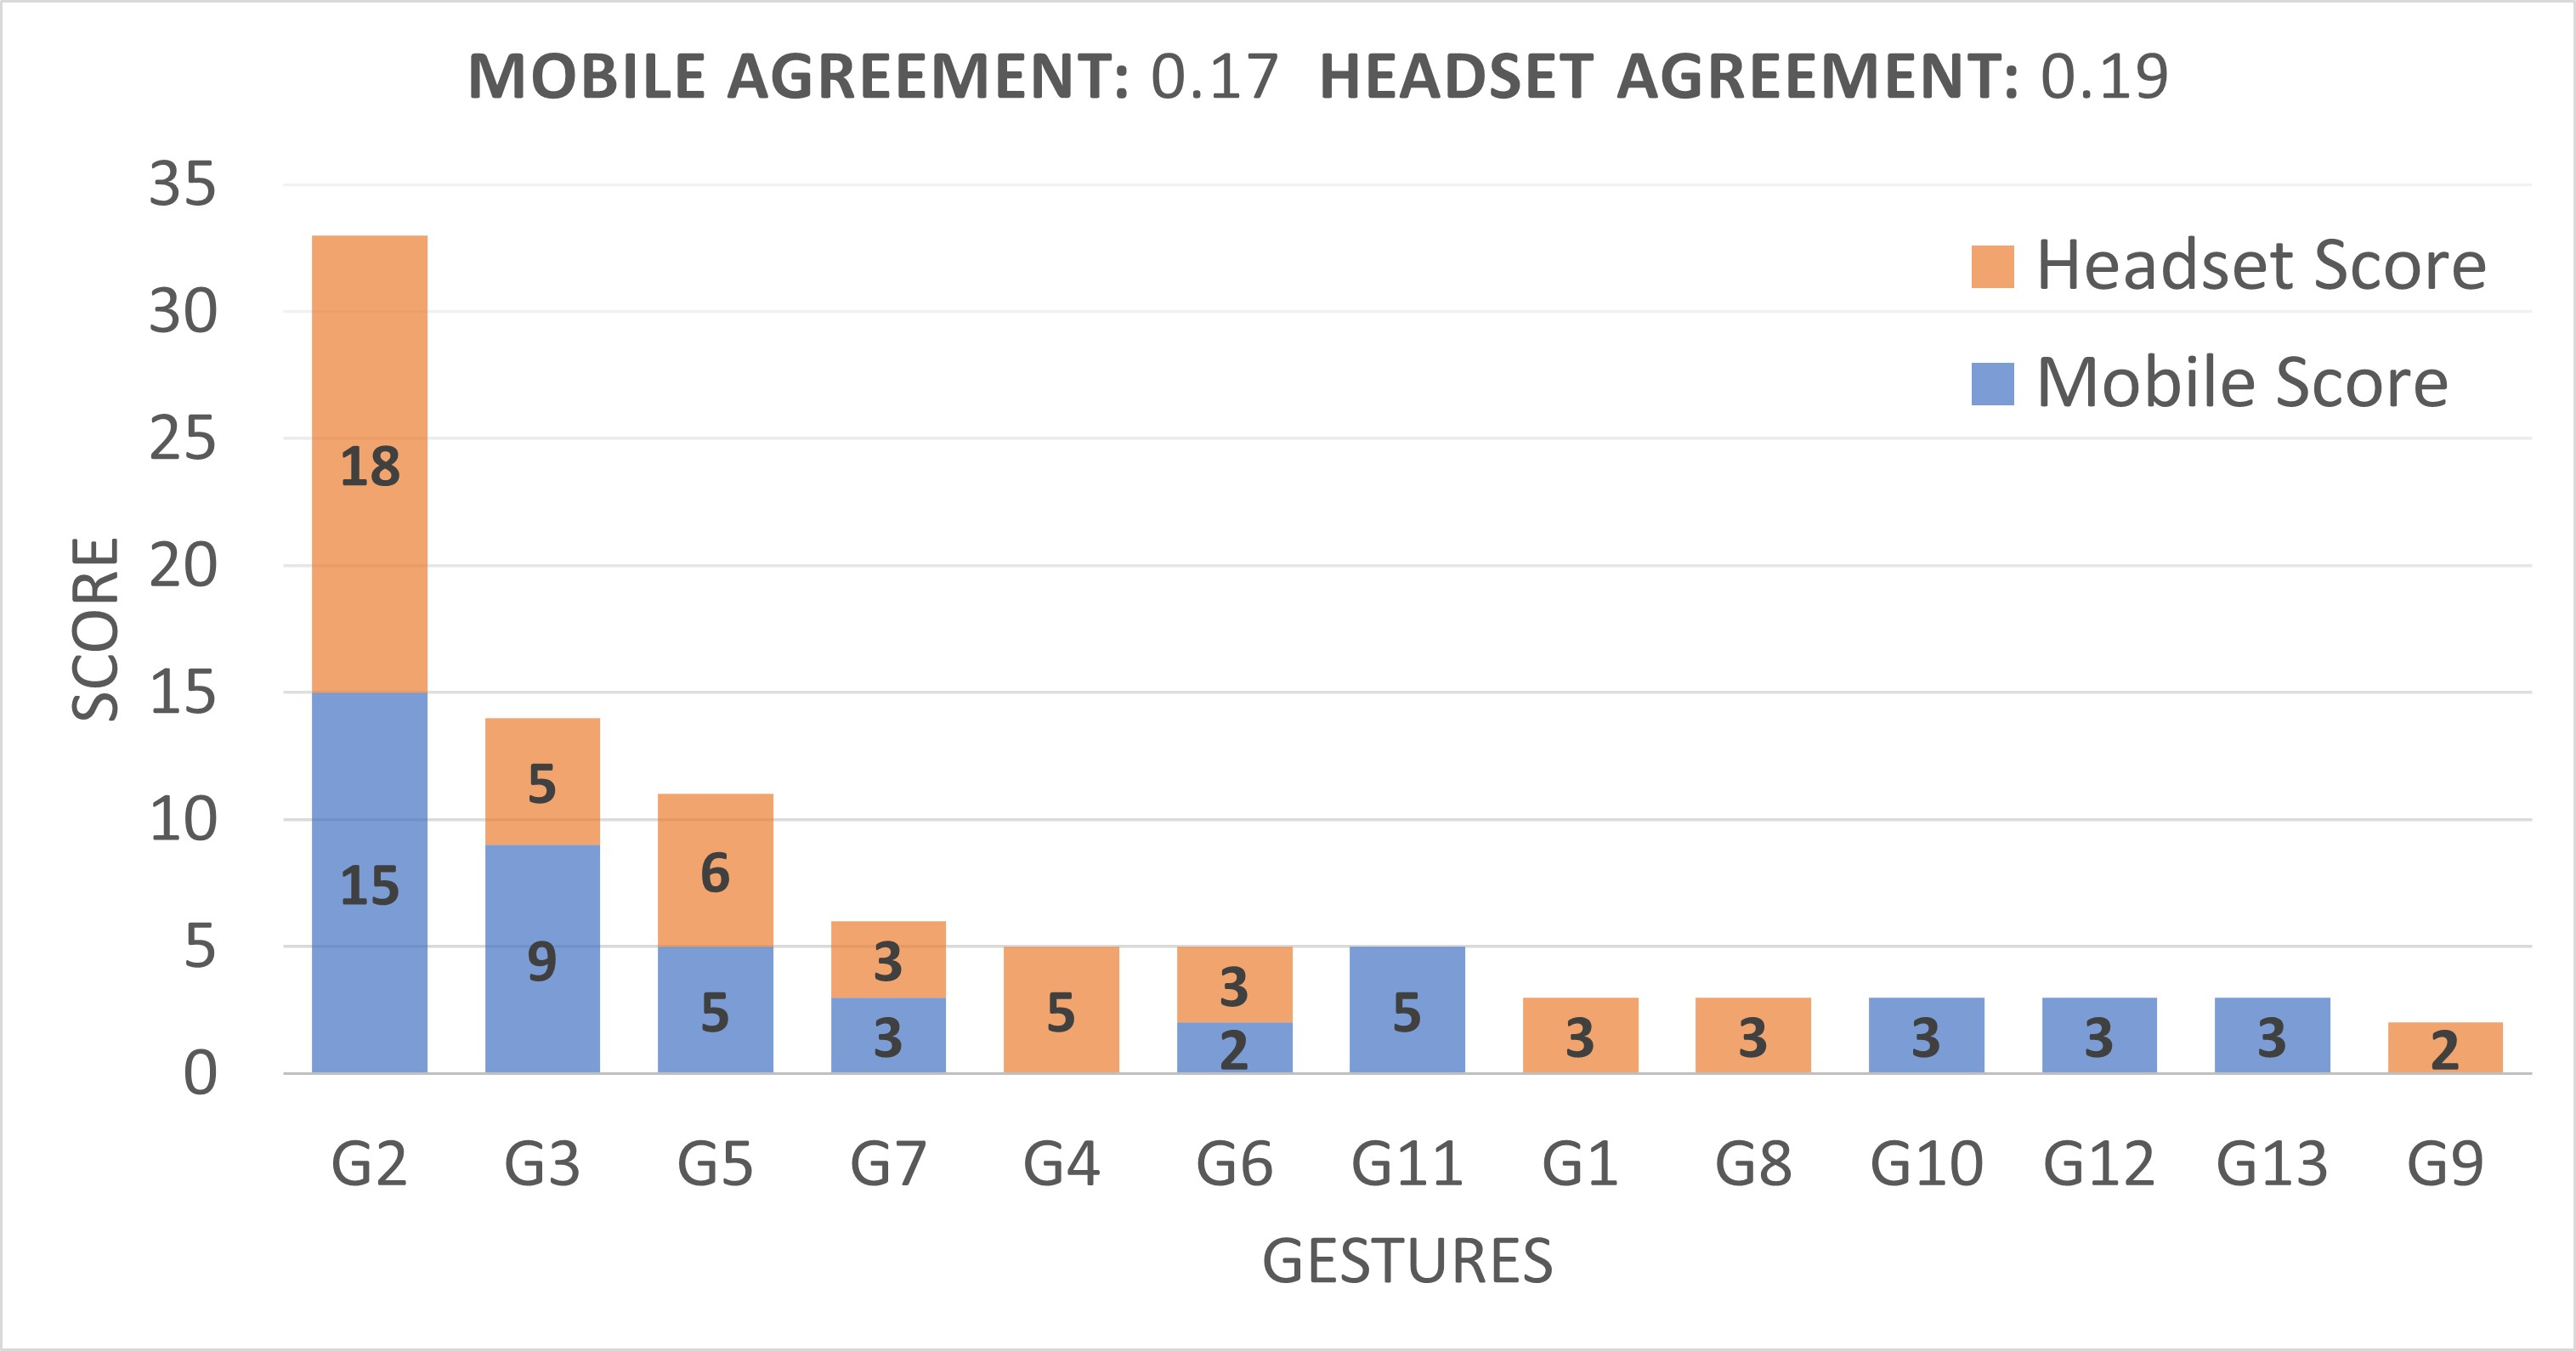
\includegraphics[alt={Figure 5.8},width=0.99\textwidth]{figures/F5-8.jpg}}
    \caption{Agreement scores for unique gestures in Task 3 \label{fig:5-8}}
\end{figure}

To wrap up the analysis of the pointing category, it was observed that users defaulted to pointing objects using an air gesture with either the index or the whole hand. Users also commonly
referred to their previous experience with touch screens, with a tap in the air or the screen that felt natural. There was not much difference between pointing digital or physical objects,
but several participants had second thoughts and concerns when pointing people, considering the index gesture as rude or inappropriate.

Task 4 required to hold and manipulate an object and was designed to examine how the two scenarios would influence the participants' interaction proposal, especially considering that
Scenario 2 provided the freedom to use both hands. There were indeed instances of gestures only appearing in Scenario 1 and others only in scenario 2. The use of mobile phones led some
participants to default to a familiar drag gesture over the screen to hold and move the digital object.

On the other hand, the headset scenario strongly promoted the participants to use the perceived physicality of the digital object to try and grasp its contour using the index finger and
thumb or even with the whole hand, as shown in Figure \ref{fig:5-9}. The next most popular gesture used a simpler approach of grasping the object by completely closing the hand over it or
pinching it with the index and the thumb. Scenario 2 appeared to promote participants to select the most complex yet more realistic approach.

\begin{figure}
    \centering{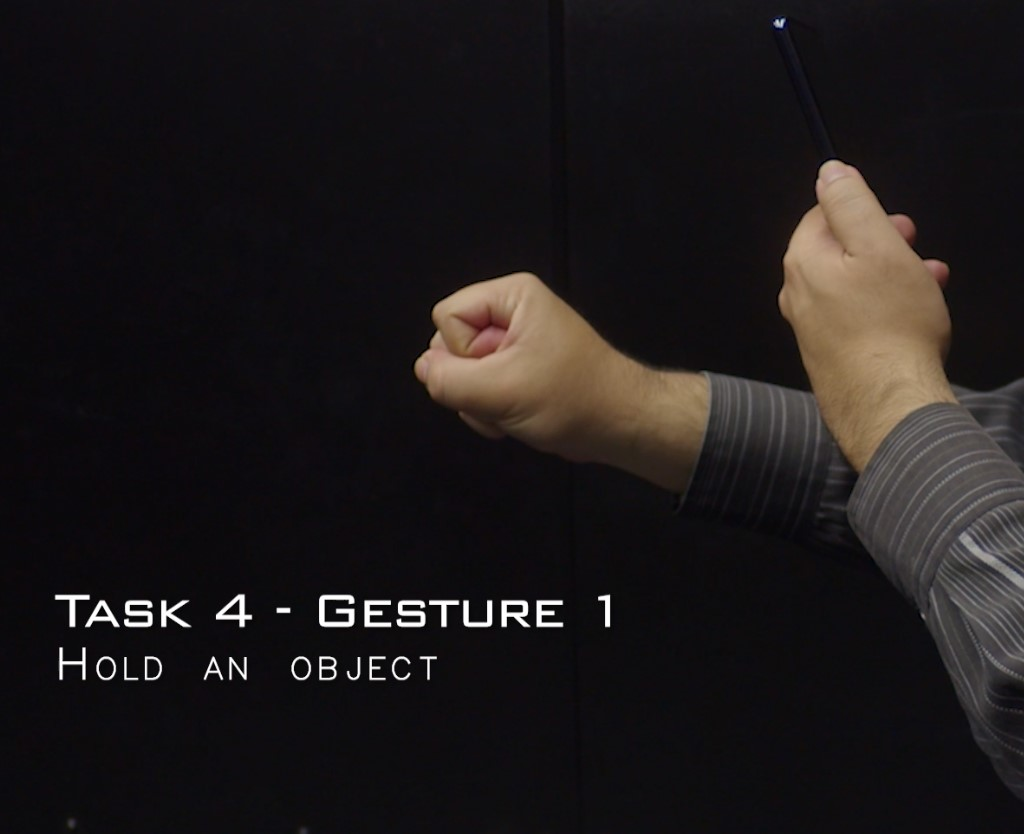
\includegraphics[alt={Figure 5.9a},width=0.3\textwidth,height=0.3\textheight]{figures/F5-9A.jpg}}
    \centering{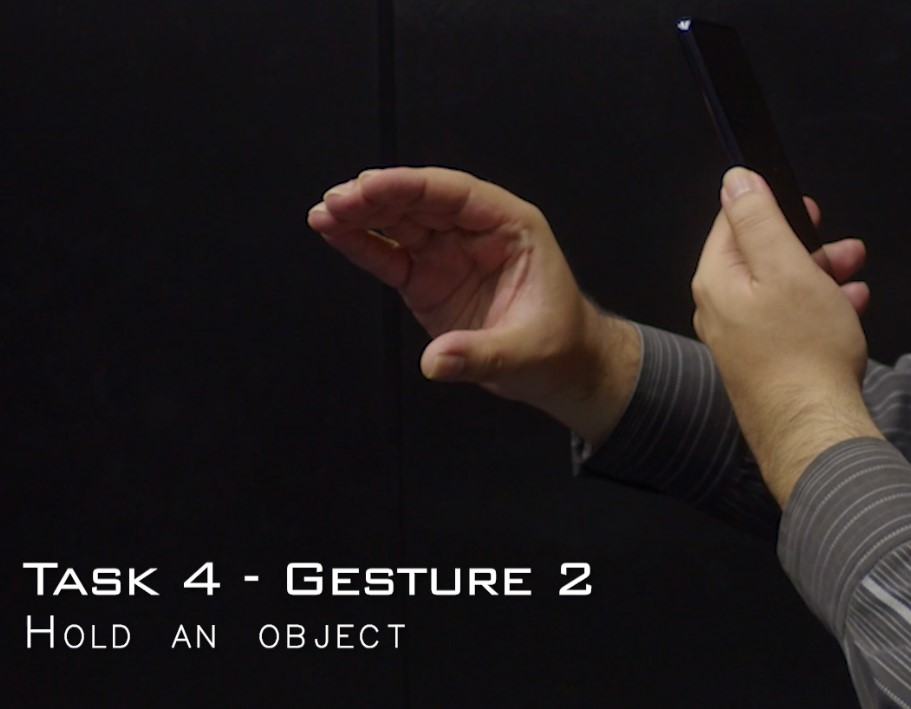
\includegraphics[alt={Figure 5.9b},width=0.3\textwidth,height=0.3\textheight]{figures/F5-9B.jpg}}
    \centering{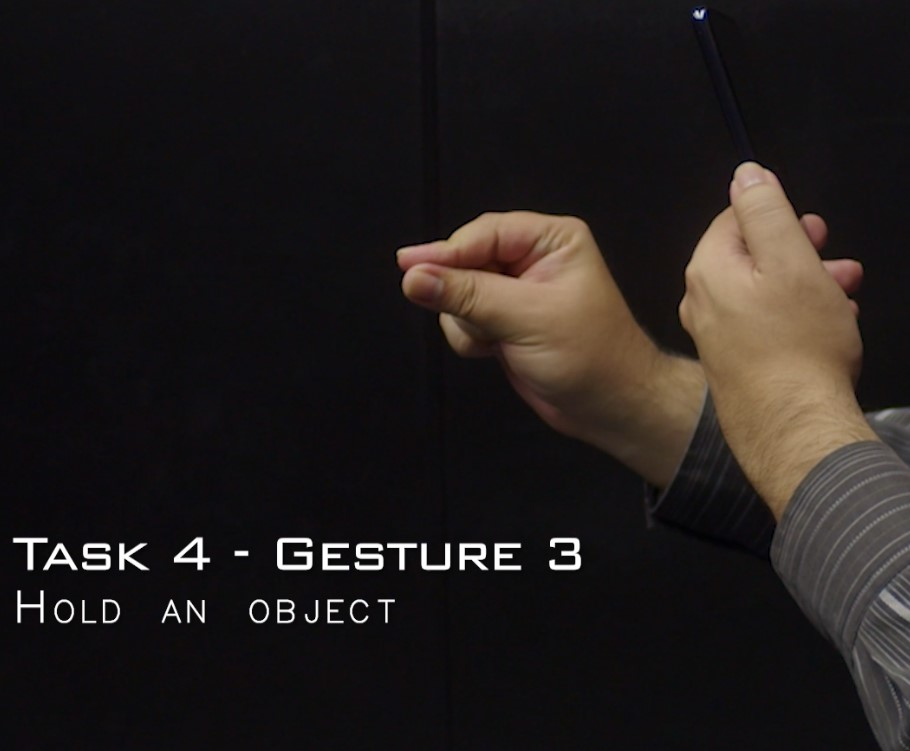
\includegraphics[alt={Figure 5.9c},width=0.3\textwidth,height=0.3\textheight]{figures/F5-9C.jpg}}
    \caption{Hold an Object - Closed Fist (left), Contour (middle) and Pinch (right) gestures \label{fig:5-9}}
\end{figure}

Task 5 is the collaborative take of the object manipulation category and was designed mostly for gathering ideas from the users on how to organise the group while manipulating objects. The
participants were specifically prompted to explain how they would share a held object or the act of sharing anything in general. In this case, both scenarios converged to the gesture of
extending an open hand in the direction of the intended target, either to automatically trigger the sharing action (a very straightforward, abstract action) or as the first step of a
process, expecting the other team member to extend their hand and take the object (a more realistic, physical action). Mobile users also converged to the motion of throwing by swiping the
object in the tocuhscreen in the direction of the intended target. Examples of all these gestures can be seen in Figure \ref{fig:5-10}.

\begin{figure}
    \centering{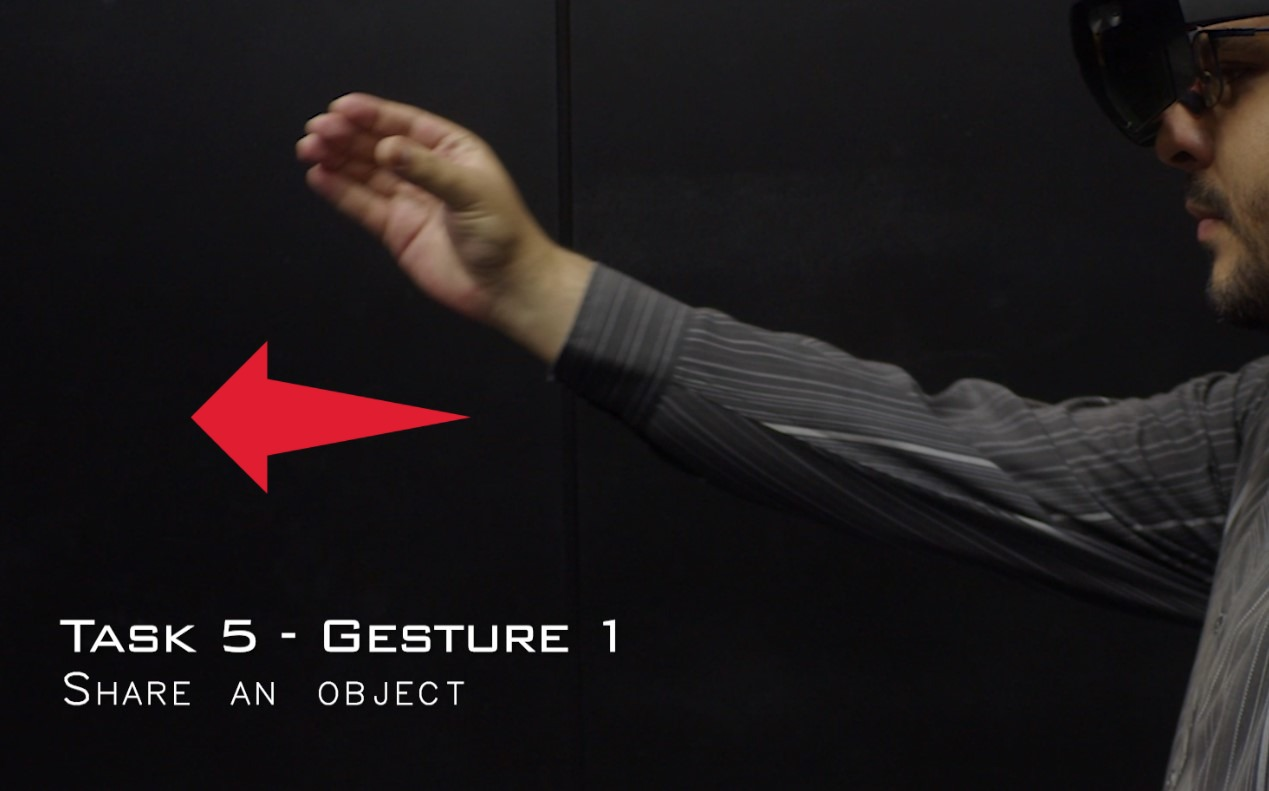
\includegraphics[alt={Figure 5.10a},width=0.49\textwidth,height=0.33\textheight]{figures/F5-10A.jpg}}
    \centering{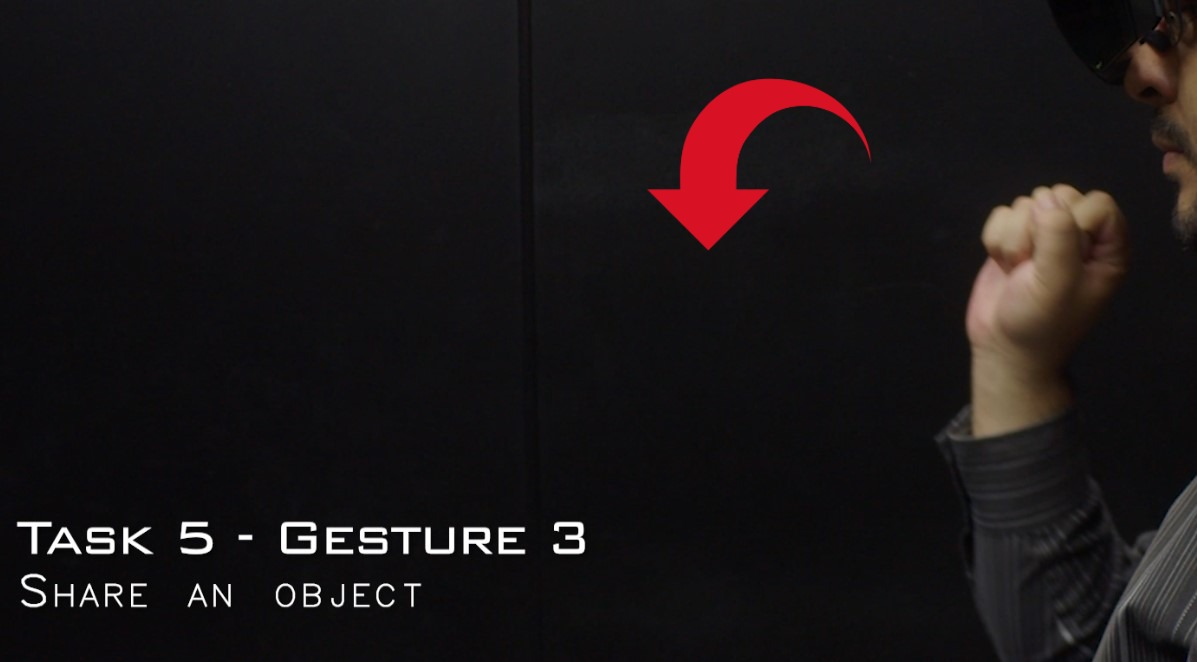
\includegraphics[alt={Figure 5.10b},width=0.5\textwidth,height=0.33\textheight]{figures/F5-10B.jpg}}
    \caption{Share an Object - Pass over (left) and Toss (right) gestures \label{fig:5-10}}
\end{figure}

For these gestures related to sharing and manipulating objects the participants proposed increasingly more complex gestures requiring full movements or patterns to convey the intended
meaning (which are harder to show in static figures). Movement ranged from simple patterns like swipes or tosses that only required a direction or a reference to the target team member,
while others proposed complex series of movements normally involving the other user in the action, with specific protocols required to initiate the sharing of an object and its receipt
from the second user. Figure \ref{fig:5-11} shows the agreement scores for all the gestures identified in Tasks 4 and 5.

\begin{figure}
    \centering{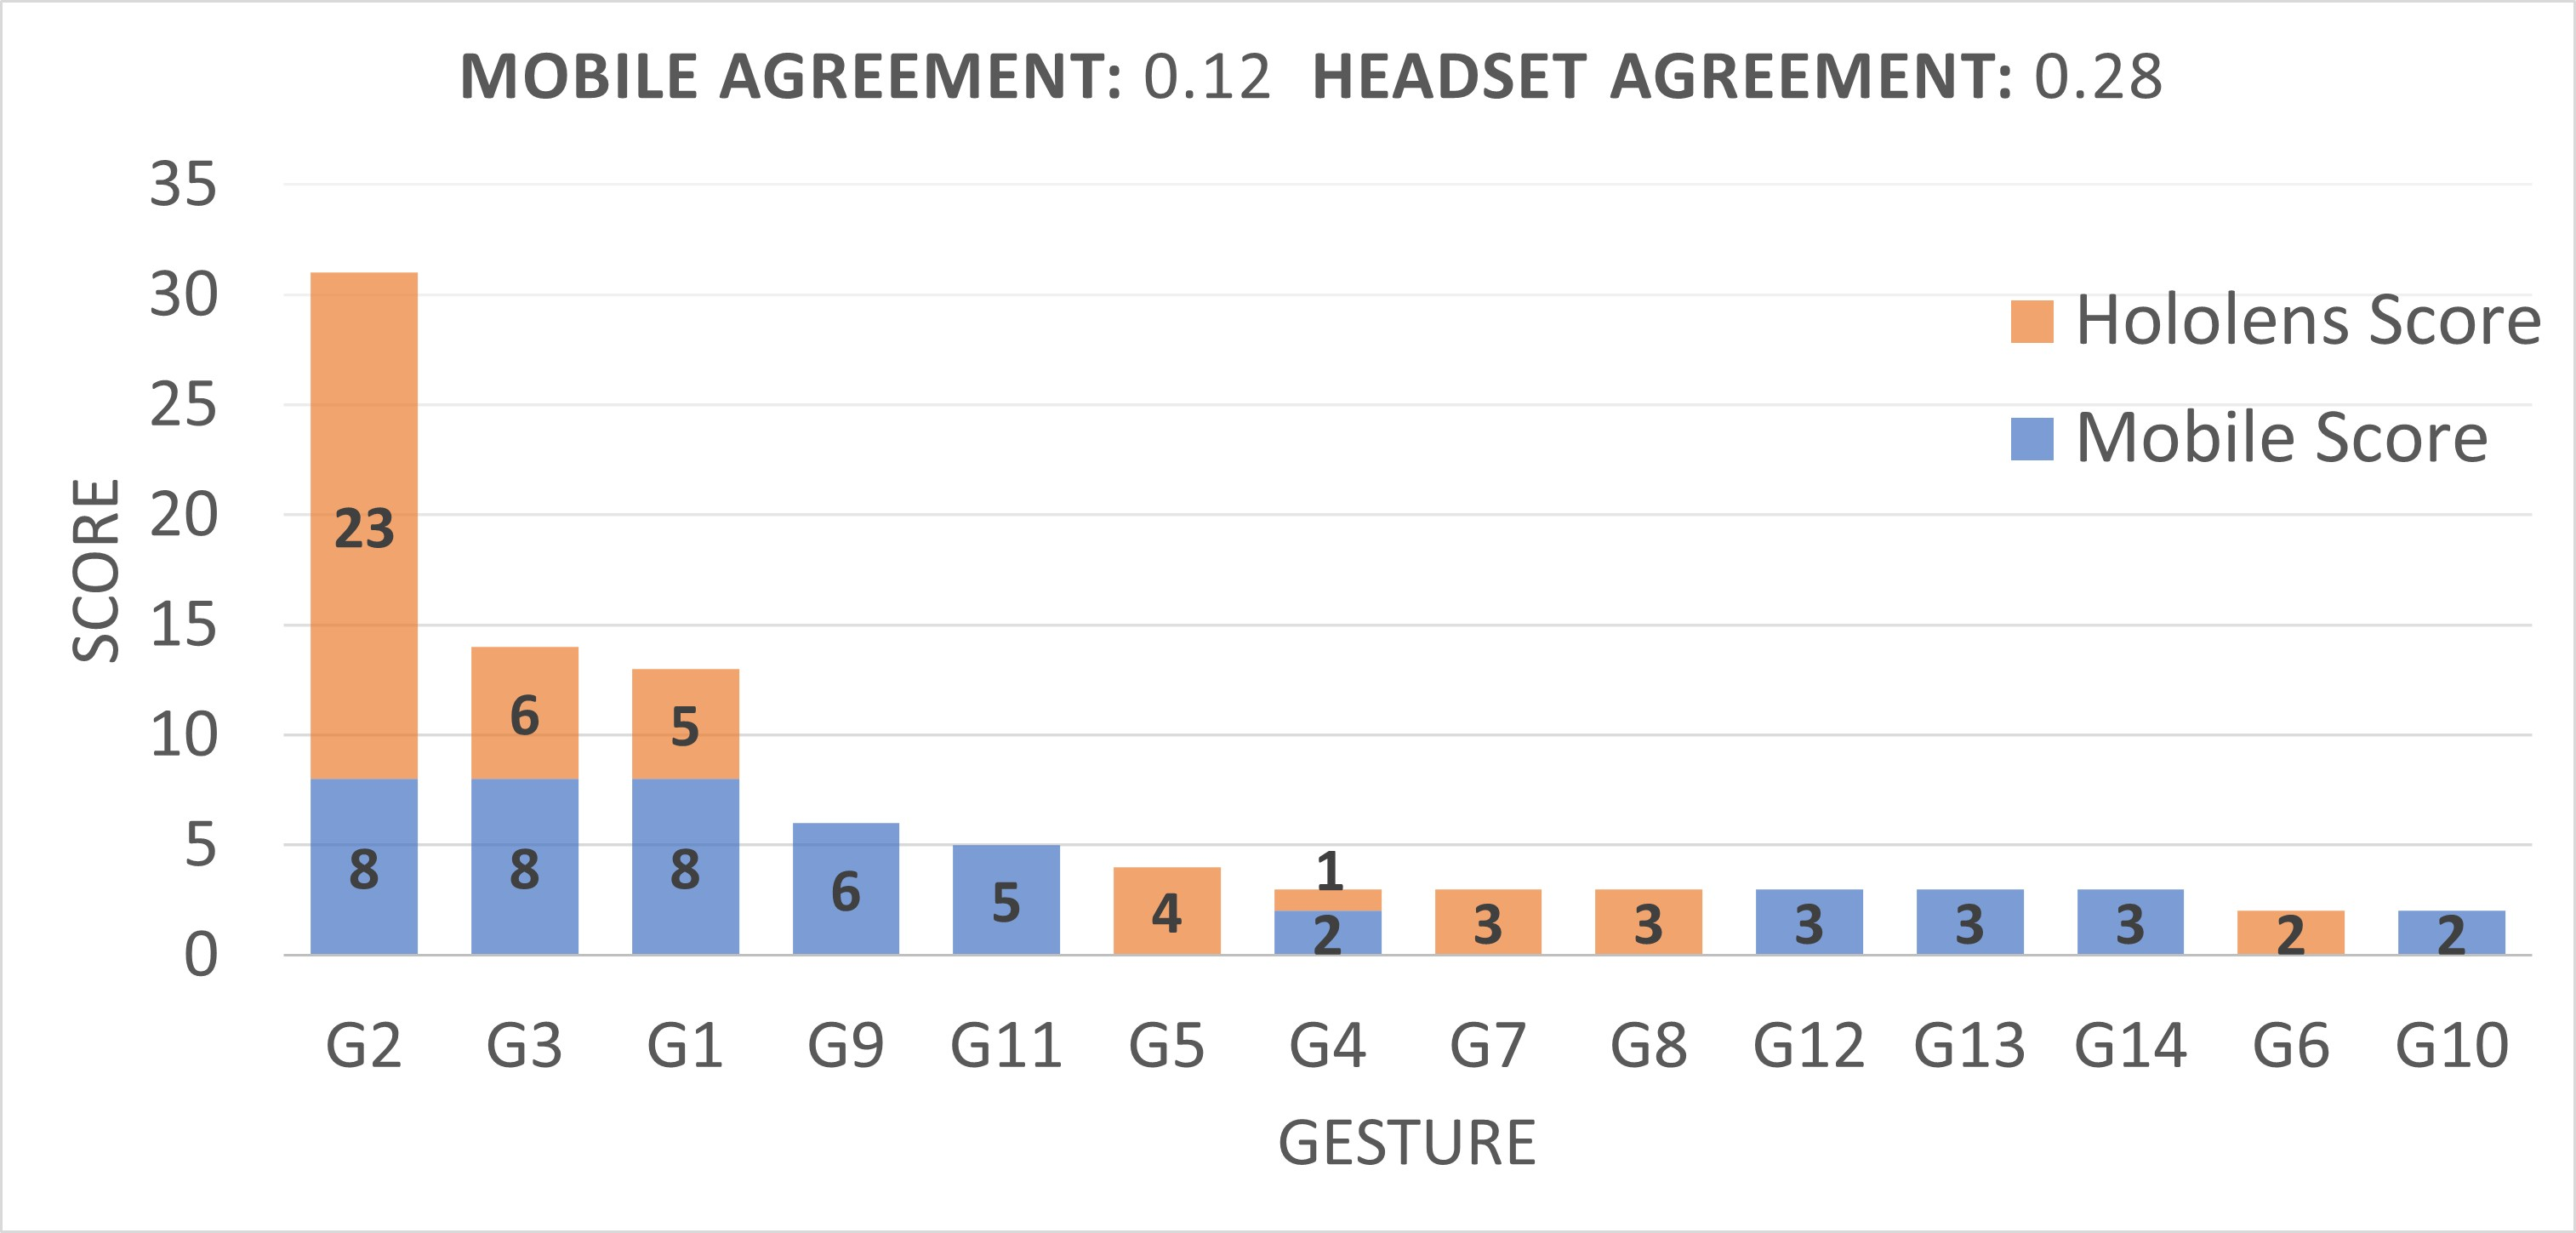
\includegraphics[alt={Figure 5.11a},width=0.99\textwidth]{figures/F5-11A.jpg}}
    \centering{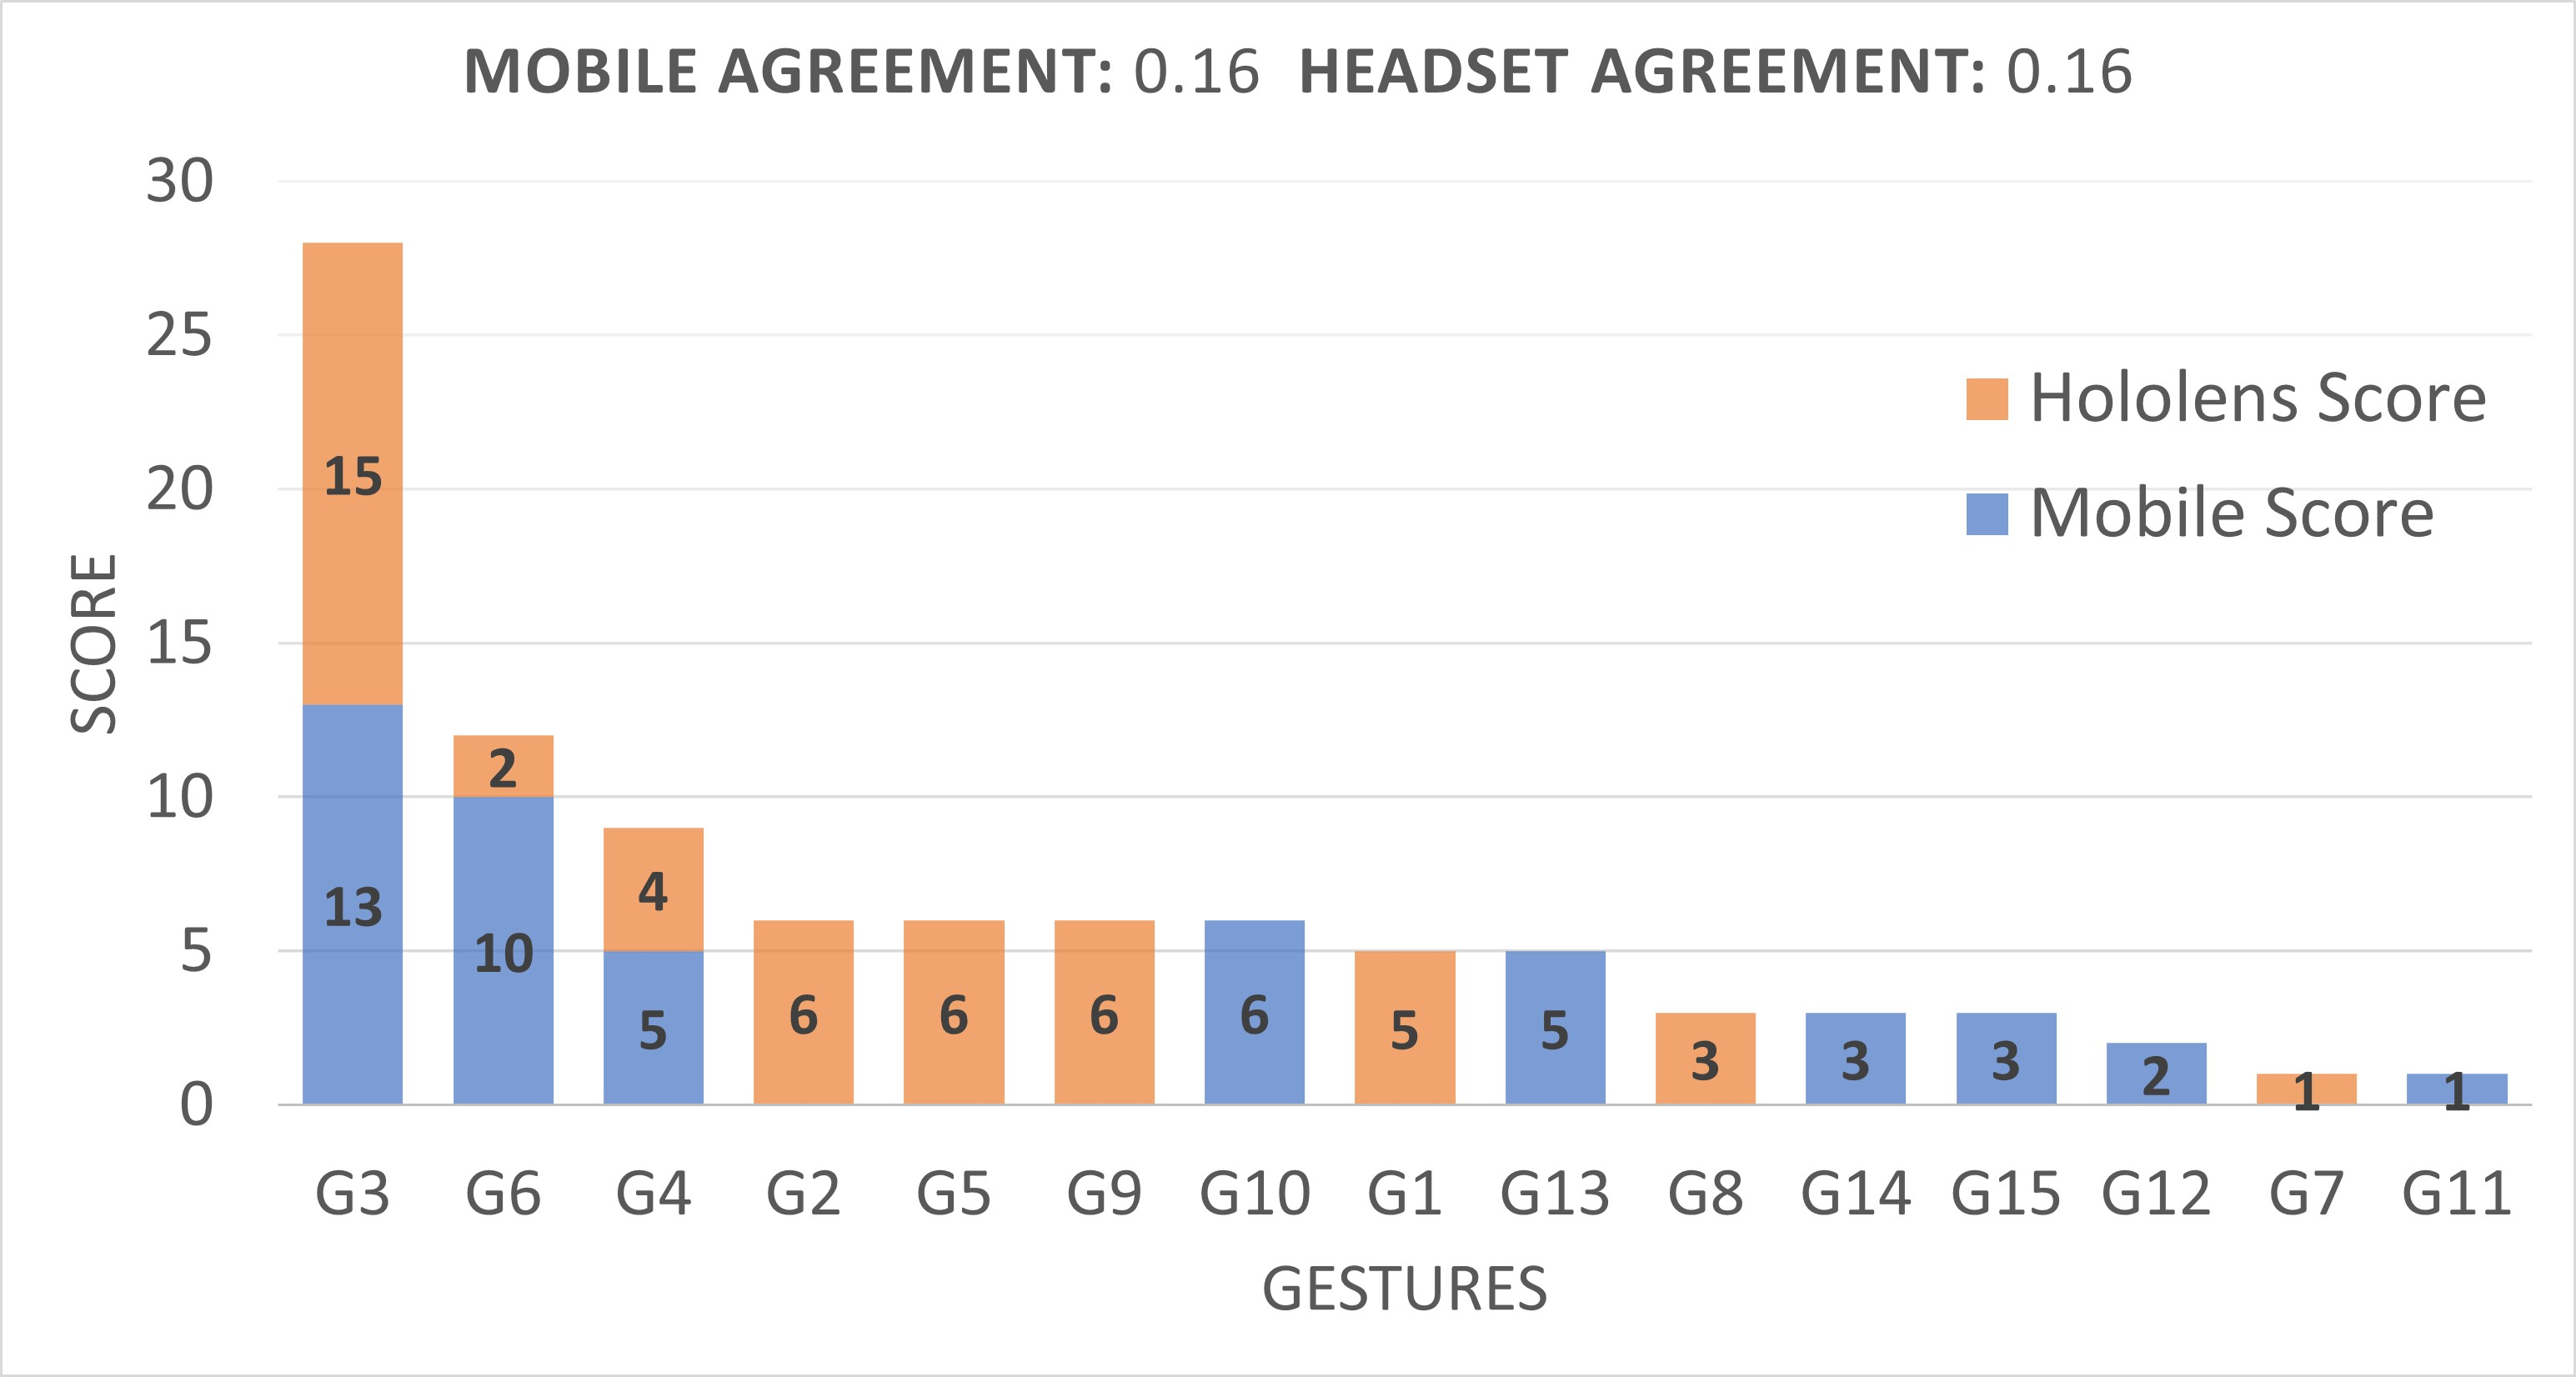
\includegraphics[alt={Figure 5.11b},width=0.99\textwidth]{figures/F5-11B.jpg}}
    \caption{Agreement scores for unique gestures in Task 4 (top) and Task 5 (bottom) \label{fig:5-11}}
\end{figure}

Tasks 6 and 8 corresponded to taking an object in and out of the \emph{private workspace} of the participants. The shared and public space metaphor was an interesting concept that appeared
in literature to emphasise the need to differentiate between public and private spaces in shared experiences. The shared versus \emph{private workspace} creates a boundary for each user to be
able to keep work and experimentation as private work and be able to control what is shared with the team and what is not. In terms of interaction design it also offered the opportunity to
understand how users would understand this concept, if at all, and if it was possible to converge into a set of gestures to represent possible actions needed for this scenario. It was
decided to focus on the process of moving from and into the private space and how can this be signalled in the shared experience. In this case, both data gathering scenarios clearly
converged to different gestures.

Both converged sets were similar in nature and consisted of moving the object with one hand to and from the area shown to participants as their \emph{private workspace}. The difference
appeared when participants in the mobile scenario saw a zone in the border of the phone's screen and dragged the object there using a hold-and-drag gesture. Few people took the object with
their hand, and if they did, they did not consistently use the same gesture proposed in Task 4.

On the other hand, headset users saw a zone in their physical space and moved the object there, sometimes holding it using the exact same gesture proposed in Task 4, but not consistently.
Other times they would use a completely different gesture to hold and drop the object or would use a different one related more to push the object into the zone or drag it close to their
own person. Figure \ref{fig:5-12} shows examples of the converged gestures for both tasks.

\begin{figure}
    \centering{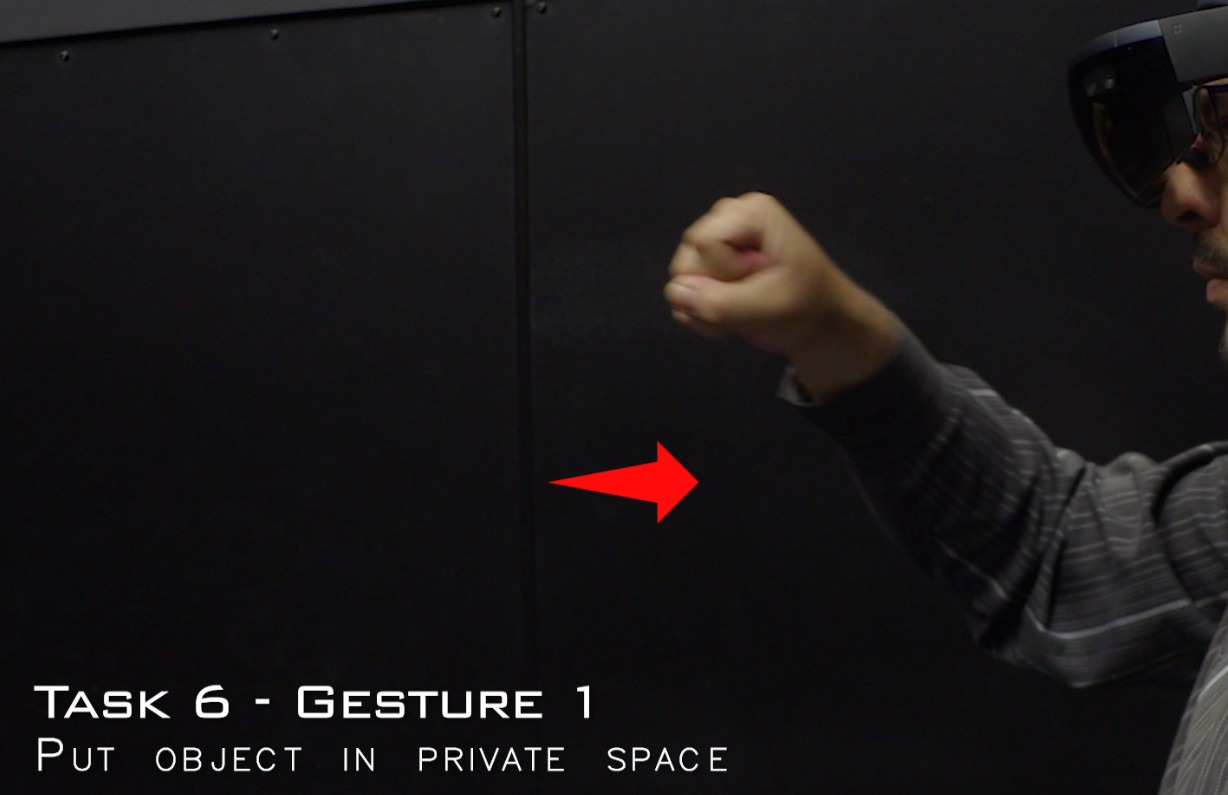
\includegraphics[alt={Figure 5.12a},width=0.3\textwidth,height=0.3\textheight]{figures/F5-12A.jpg}}
    \centering{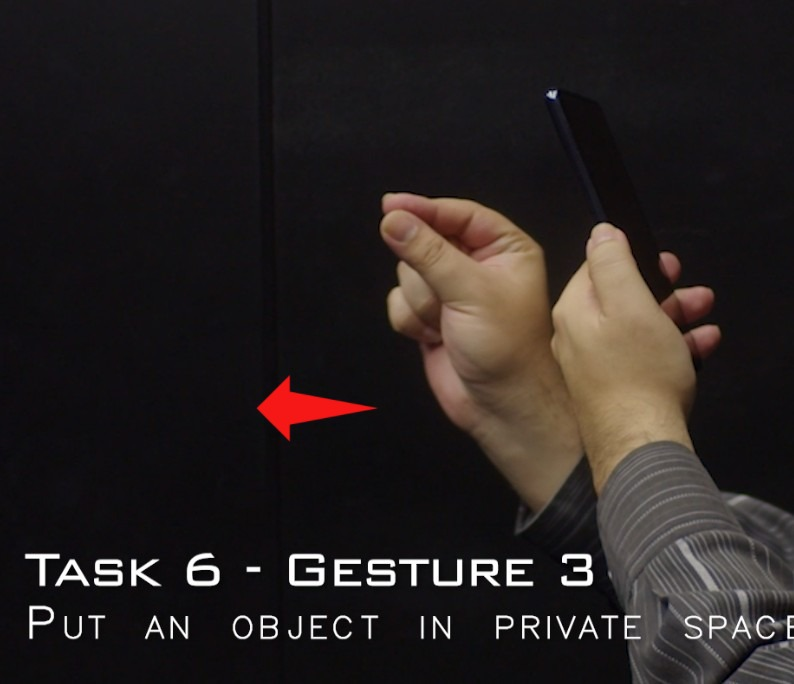
\includegraphics[alt={Figure 5.12b},width=0.3\textwidth,height=0.3\textheight]{figures/F5-12B.jpg}}
    \centering{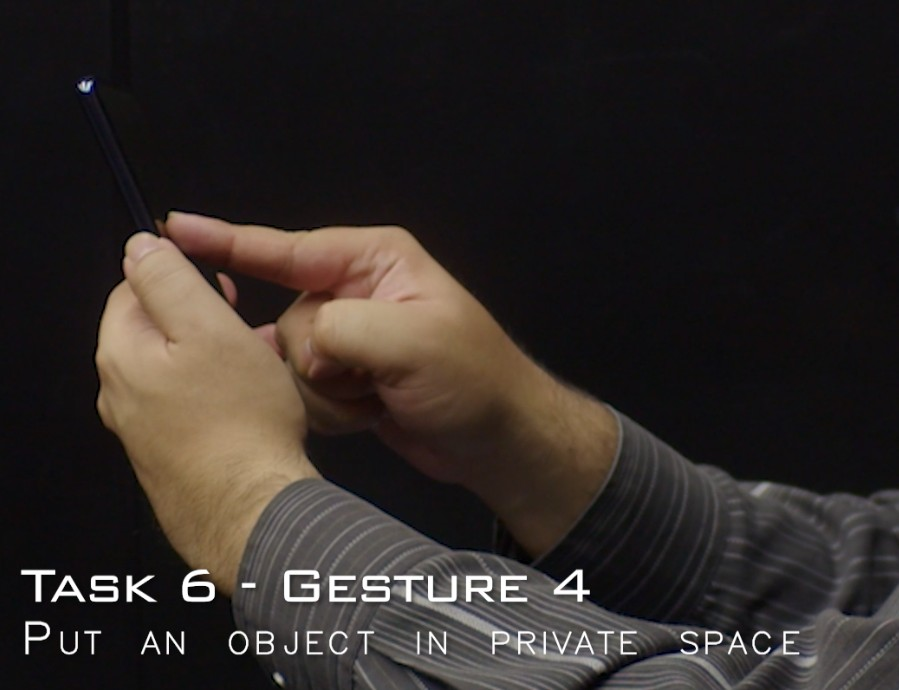
\includegraphics[alt={Figure 5.12c},width=0.3\textwidth,height=0.3\textheight]{figures/F5-12C.jpg}}
    \caption{Put an Object in Private Space - Fist hold Inwards (left), Pinch Hold Inwards (middle) and Screen Swipe (right) gestures \label{fig:5-12}}
\end{figure}

This distinction between scenarios is very probable due to the way the private workspace was shown in each scenario: a 2D space on the screen for Scenario 1 and a 3D area near the user for
Scenario 2. This could have prompted the participants to use the screen rather than an air gesture. It is also probable that the screen interaction would have been one of the most
prominent results even if both scenarios would have shown the same representation of the tasks, considering how for tasks 4 and 5 mobile users also defaulted to interactions using the
screen despite the mostly 3D representation shown to them in the application.

The idea behind Task 7 was not necessarily collaborative in nature, mostly exploring a common action in any other software that could be expected by users in the functionality of \emph{WorkshopAR}.
Its implications in the coordination of action when manipulating objects could also be discussed. In the end, Task 7 represented one of the less agreed upon sets, and showed a variety of
approaches to signal the process of undoing the previous action, but the most agreed upon comment among both scenarios was that such an action could better be implemented via a button or
option in a menu, and not linked to a gesture, either in the air or the touch screen. This is important because the idea of unnecessary gestures became more prevalent in the following tasks.
Figure \ref{fig:5-13} shows some of the most common gestures proposed for the task, while figure \ref{fig:5-14} shows the distribution of the agreement score for all 22 gestures identified.

\begin{figure}
    \centering{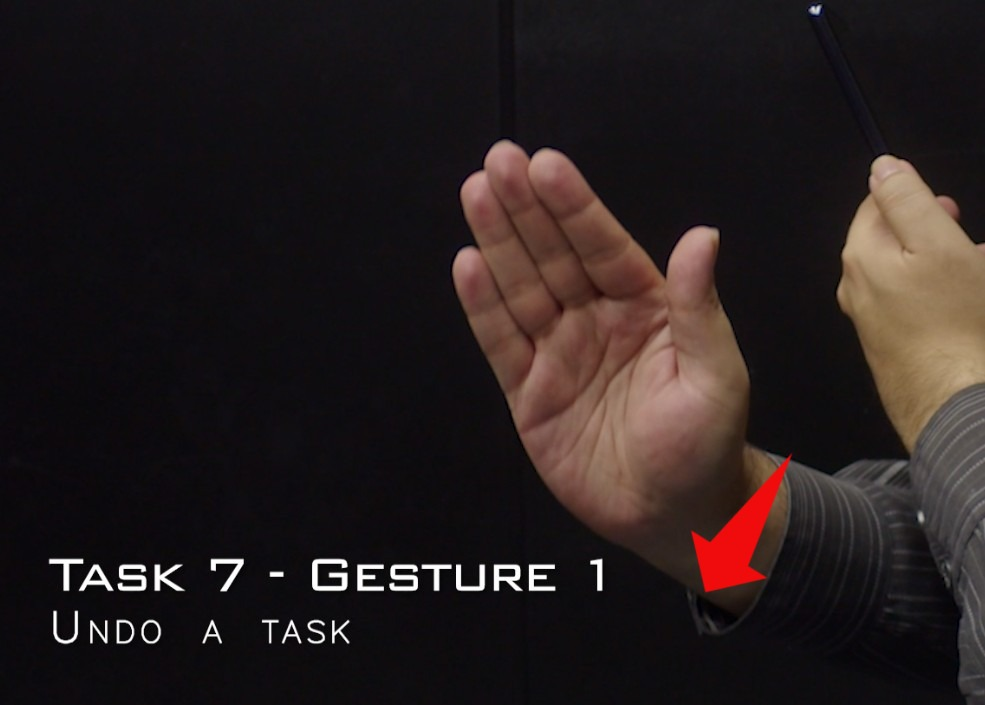
\includegraphics[alt={Figure 5.13a},width=0.49\textwidth,height=0.33\textheight]{figures/F5-13A.jpg}}
    \centering{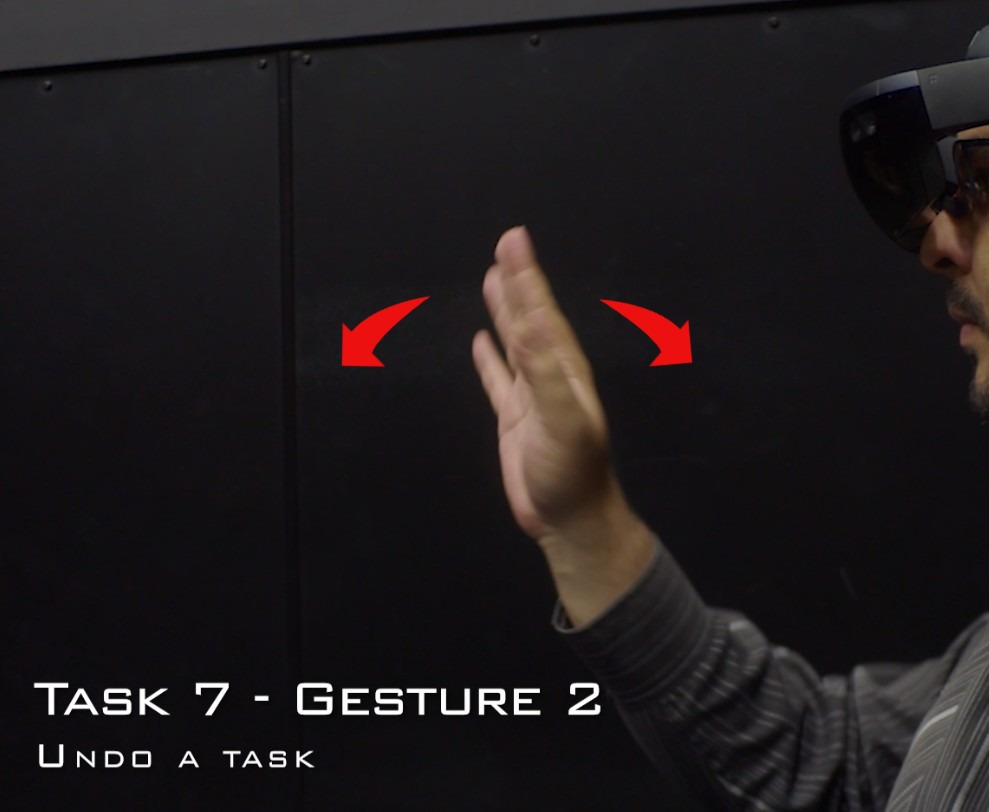
\includegraphics[alt={Figure 5.13b},width=0.5\textwidth,height=0.33\textheight]{figures/F5-13B.jpg}}
    \caption{Undo a Task - Push Sideways (left) and Wave (right) gestures \label{fig:5-13}}
\end{figure}

\begin{figure}
    \centering{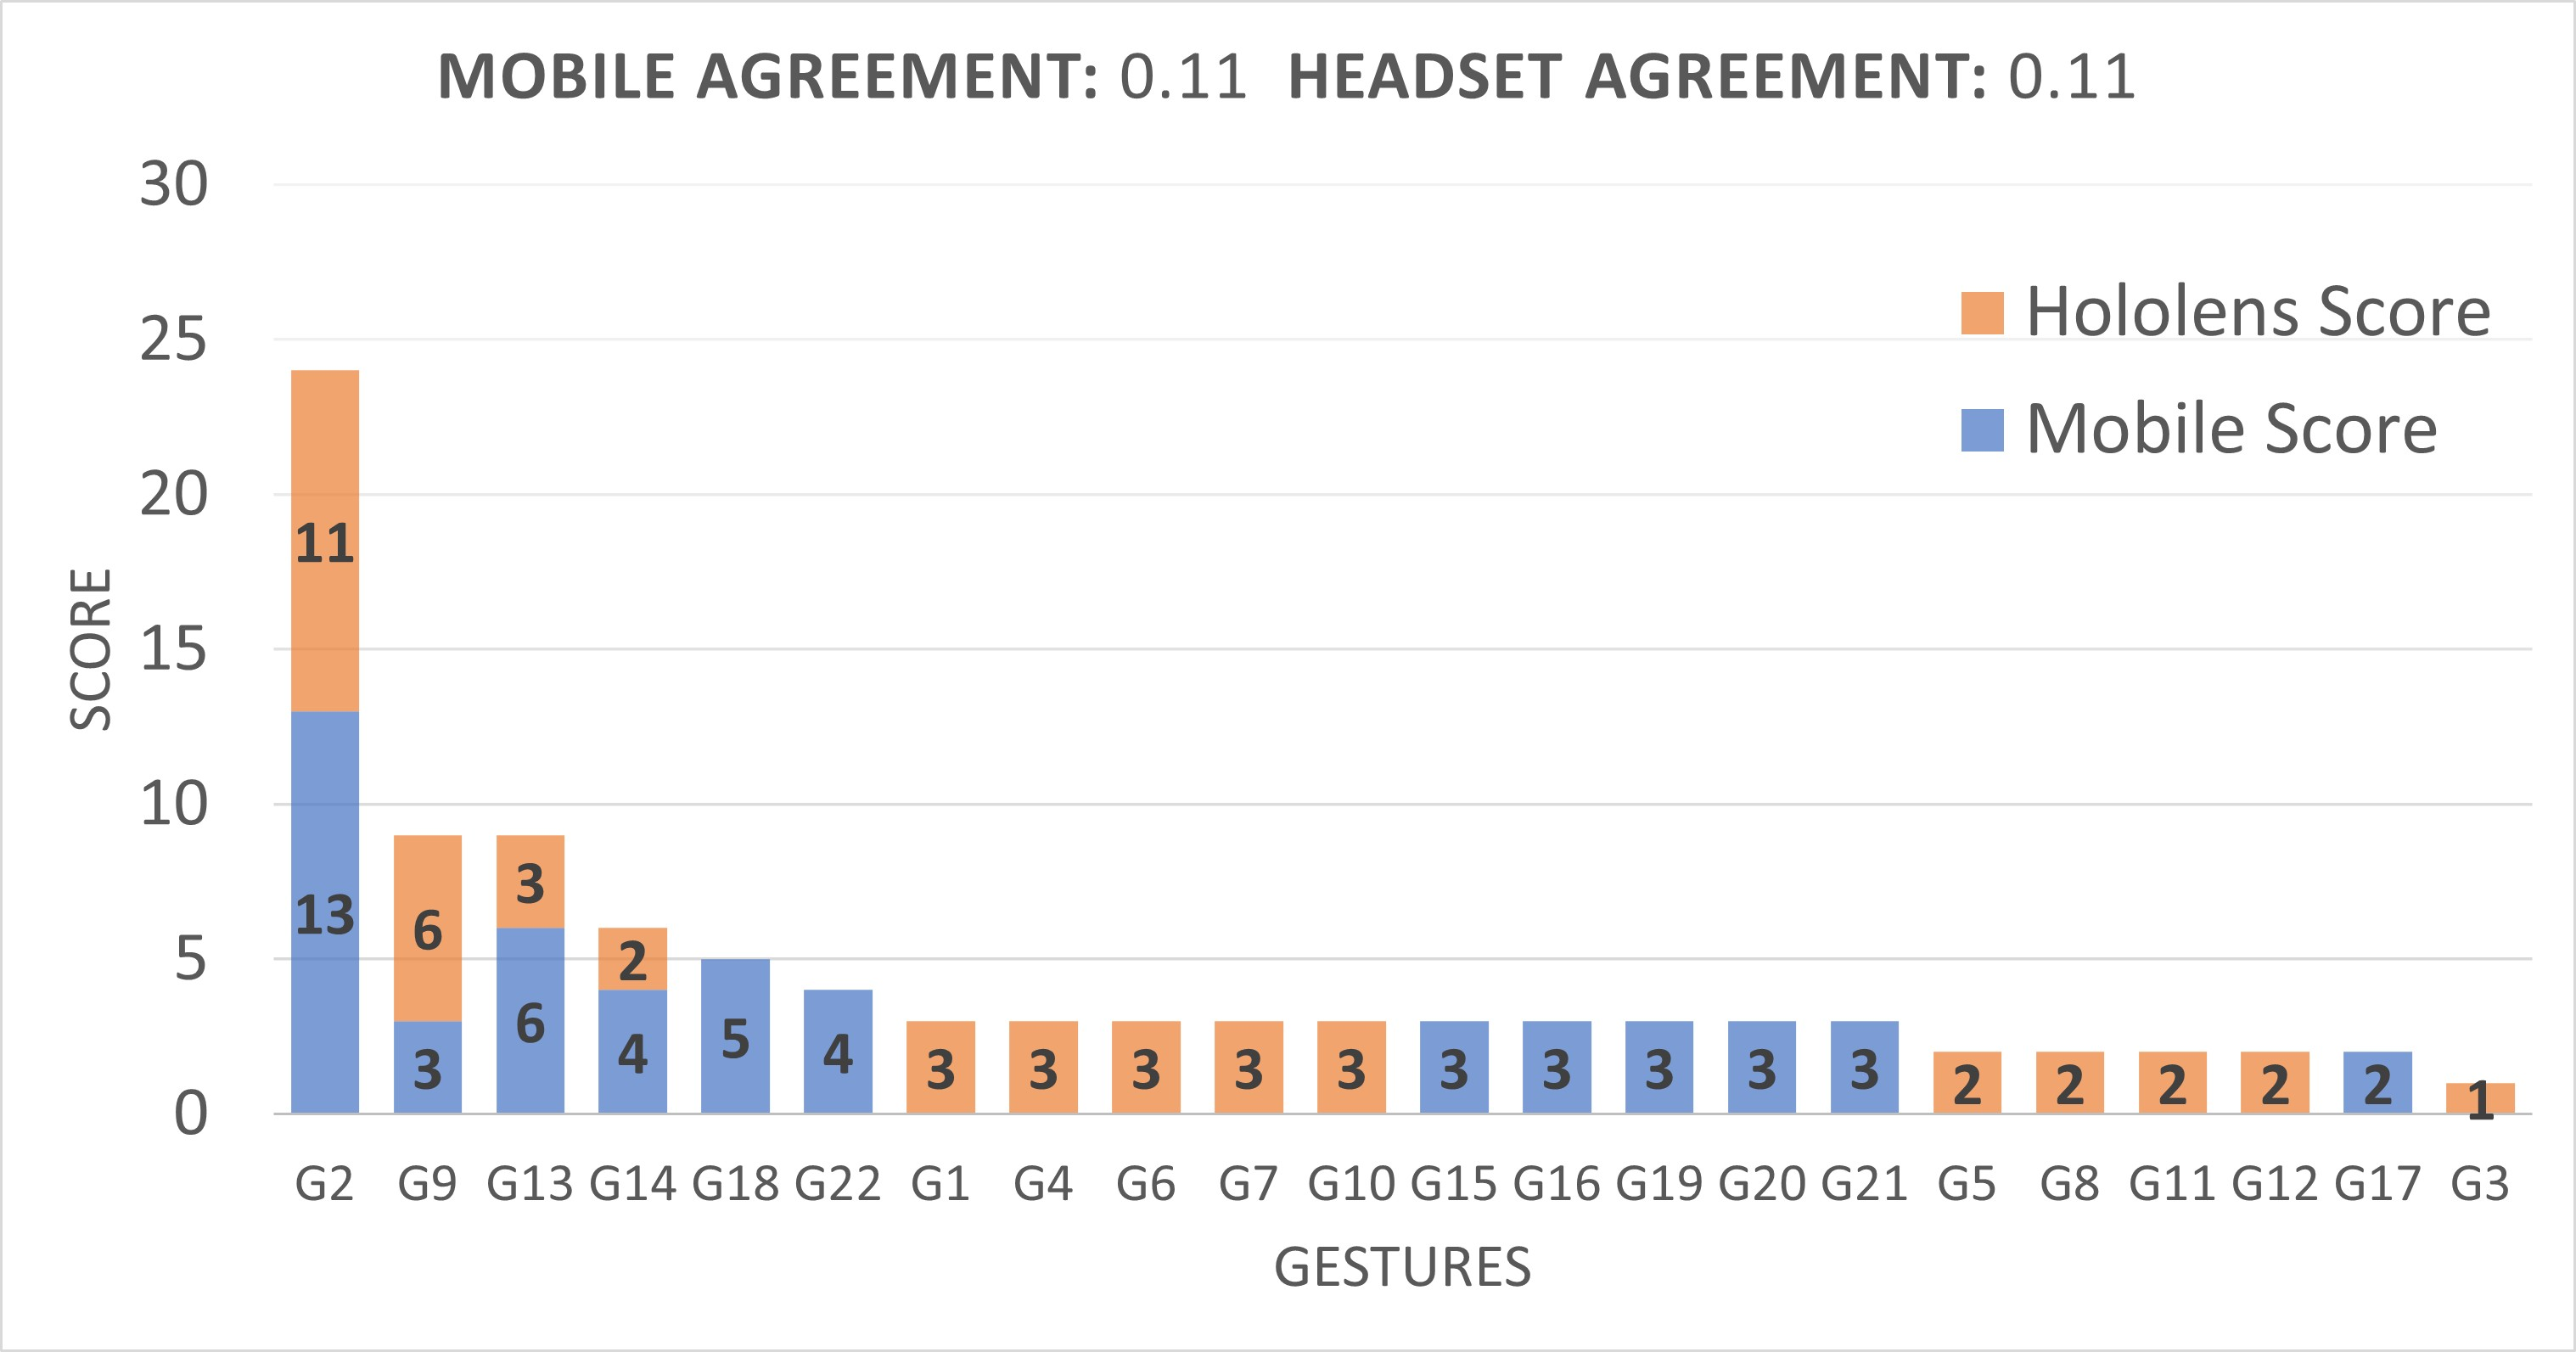
\includegraphics[alt={Figure 5.14},width=0.99\textwidth]{figures/F5-14.jpg}}
    \caption{Agreement scores for unique gestures in Task 7 \label{fig:5-14}}
\end{figure}

Tasks 9 and 10 asked the participants to vote in a debate or answer a multiple-choice question. The tasks were designed to identify differences in interaction when the participants had to
deal with a clear user interface in comparison to a more physical selection involving objects in the digital space. A similar situation to that of tasks 6 and 8 appeared here when
presenting to the users a more physical representation of the tasks in comparison to one mostly based in UI. Within these tasks, results were consistent, and participants in Task 10
proposed more air gesture and with more complexity.